\documentclass[twoside,openright]{report}

\usepackage{graphicx}
\usepackage{amsmath,amssymb,amsthm}
\usepackage{dsfont}
\usepackage[top=3cm,bottom=3.5cm,left=3.5cm,right=3cm]{geometry}
\usepackage{caption}
\usepackage{subcaption}
\usepackage{footnote}
\usepackage[hidelinks]{hyperref}

\makesavenoteenv{tabular}
\makesavenoteenv{table}

\usepackage{array}
\newcolumntype{N}{@{}m{2pt}@{}}

\newcommand\PS[2]{\left \langle #1 \right \rangle_{#2}}
\newcommand\N[2]{\left| \left| #1 \right| \right|_{#2}}
\DeclareMathOperator*{\Var}{var}
\DeclareMathOperator*{\E}{E}
\DeclareMathOperator*{\Cov}{cov}
\makeatletter
\newcommand{\shorteq}{%
  \settowidth{\@tempdima}{a}% Width of hyphen
  \, \resizebox{\@tempdima}{\height}{=} \,%
}
\makeatother


\newcommand\todo[1]{\textbf{TODO: #1}}
\newcommand\dx{\, d}

\newtheorem{definition}{Definition}
\newtheorem{theorem}{Theorem}
\newtheorem{property}{Property}
\newtheorem{example}{Example}

\author{N. Durrande}
\date{Mines St-\'Etienne -- Data Science -- 2015/2016}
\title{Lecture notes on Gaussian process regression}

\linespread{1.2}
\begin{document}
\maketitle	


\tableofcontents

%%%%%%%%%%%%%%%%%%%%%%%%%%%%%%%%%%%%%%%%%%%%%%%%%%%%%%%%%%%%
%%%%%%%%%%%%%%%%%%%%%%%%%%%%%%%%%%%%%%%%%%%%%%%%%%%%%%%%%%%%
\chapter*{Introduction}
\addcontentsline{toc}{chapter}{Introduction}

\section*{Context}
\addcontentsline{toc}{section}{Context}

\paragraph{}
Acquiring data usually comes with a cost and, quite often, this cost puts a limit to the number of data available. This is for example the case when the data comes from a physical experiment: time or budget limitations put a limit to the number of experiments and one has to chose carefully the ones to run depending on the aim of the study. Nowadays, the increasing computational power allows to replace more and more physical experiments by numerical simulations (hence the name experiment \emph{in silico}) but one part of the problem stays unchanged: even if experiments do not require any prototyping nor specific equipment, the complexity of the models implies a large computation time for each simulation run and it is quite common for finite element solvers or Monte Carlo simulators to take hours or even days before returning a result with the desired precision. Hence, the limitation on the number of experiments still stands.

\paragraph{}
In practice, a large evaluation cost for a function $f$ makes many classical methods impracticable. For example, numerical methods for computing the mean value (i.e.\@ the integral) of a function are typically based on quadrature which requires a large number of observations. In the same fashion, \emph{uncertainty propagation}, which is the study of the image of a random variable through $f$ often use Monte Carlo which is intractable in such context. \emph{Optimization} is another typical application field that is affected by the limited number of observations since most classical methods, such as gradient descent, require many functions calls. Although the aim is not to make an exhaustive list of the problems affected by evaluation cost, we cannot avoid to cite here the issue of \emph{inverse problems} such as \emph{numerical simulator calibration} where we want to retrieve some parameters values $p$ for which the numerical simulator outputs are as close as possible to a ground truth.

\paragraph{}
This call for a dedicated mathematical framework for the study of functions based on a few number of observations. Historically, the first detailed mathematical framework for this problem can be traced back to Legendre and Gauss who used least square methods to predict the movement of planets. The latter predicted in 1801 where the newly discovered dwarf planet \emph{Ceres} would reappear after it journey behind the sun, using only three observations of the past planet position. The methods we are going to detail in this document have first been studied in the 50s by the South African engineer Danie G. Krige who was interested in predicting the gold grade in a mine in the Witwatersrand. Since this date, they have received a lot of interest from the scientific community and there are now three frameworks dedicated to such problems: the first one is (geo-)statistics where we are interested in the Best Linear Unbiased Estimator (BLUE), the second one is probability with the study of random processes and the last one is functional analysis with the theory of Reproducing Kernel Hilbert Spaces (RKHS). Although all these frameworks have their own specificities, they are all based on a common ground and they all lead to very similar results. In this document, we will focus on the probabilistic approach and the theory of Gaussian processes.

\paragraph{}
The LaTeX sources of this document as well as the R scripts that have been used to generate the figures are available on the author's website: http://sites.google.com/site/nicolasdurrandehomepage.

\section*{Notations}
\addcontentsline{toc}{section}{Notations}
\paragraph{}
We will make an extensive use of vectorial notations in this document. Unless stated otherwise, lower-case variables such as $x,y$ are vectors. Random variables, matrices or processes will be denoted with upper-case such as $Y,Z$. Matrices such as a design of experiments\footnote{$n$ points in a $d$-dimensional space are written as a $n \times d$ matrix $X$.} or covariance matrices will also be represented by upper-case letters.

\paragraph{}
Furthermore, we will consider that functions can be called in a vectorial fashion: if $f$ is a function over $\mathds{R}$, then for $x_1,x_2,x_3 \in \mathds{R}$, $f((x_1,x_2,x_3))$ will be a vector of general term $(f((x_1,x_2,x_3)))_i = f(x_i)$. This can be extended to functions defined over $\mathds{R}^d$: for $f: \mathds{R}^d \rightarrow \mathds{R}$ and a $n \times d$ matrix $X$, $f(X)$ will return a column vector of length $n$. Similarly, if $g$ is a function $\mathds{R}^d \times \mathds{R}^d \rightarrow \mathds{R}$, then if $X_1$ and $X_2$ are respectively $n_1 \times d$ and $n_2 \times d$ matrices then the output of $g(X_1,X_2)$ is a $n_1 \times n_2$ matrix.

% \paragraph{}
% The inner product of an Hilbert space $\mathcal{H}$ will be denoted by $\PS{.,.}{\mathcal{H}}$. When it is not specified, we will consider the usual structures such as the Euclidean inner product over $\mathds{R}^d$. As explained previously, inner products can be called in a matrix fashion.

%%%%%%%%%%%%%%%%%%%%%%%%%%%%%%%%%%%%%%%%%%%%%%%%%%%%%%%%%%%%
%%%%%%%%%%%%%%%%%%%%%%%%%%%%%%%%%%%%%%%%%%%%%%%%%%%%%%%%%%%%
\chapter{Multivariate Gaussian and Gaussian processes}

\section{Multivariate Gaussian distribution}

\paragraph{}
A random variable follows a Gaussian (or normal) distribution with mean $\mu$ and variance $\sigma^2$ if its probability density function is
\begin{equation}
f(x) = \frac{1}{\sigma \sqrt{2 \pi}} \exp \left(-\frac{(x-\mu)^2}{2 \sigma^2} \right) \text{ for } x \in \mathds{R}.
\end{equation}  

\paragraph{}
The concept of random variables can be generalised to \emph{random vectors}, which are also called \emph{multivariate random variables}: a random vector $Y=(Y_1,\dots,Y_d)^t$ is a vector whose components are random variables defined over the same probability space. In this framework, a sample is not a scalar value but an element of $\mathds{R}^d$. The fact that the random variables are defined over the same probability space allows to study the dependencies between the elements of the vector. As for the univariate case, the concepts of moments can be generalised: if $Y$ and $Z$ are column random vectors with respective length $d$ and $n$, the expectation, variance and covariance are defined as
\begin{align}
        &\E[Y]=(\E[Y_1],\dots,\E[Y_d])^t &\qquad &\text{ this a column vector of length }d\\ 
        &\Var[Y]= \E[Y Y^t] - \E[Y] \E[Y^t] &\qquad &\text{ this a $d \times d$ matrix with entries } \Cov(Y_i,Y_j)\\ 
        &\Cov[Y,Z]= \E[Y Z^t] - \E[Y] \E[Z^t] &\qquad &\text{ this a $d \times n$ matrix with entries } \Cov(Y_i,Z_j).
\end{align}
A direct consequence of the definition of $\Cov[Y,Z]$ is that for any matrices $A$ and $B$ with respective number of columns equal to $d$ and $n$, we have $\Cov[AY,BZ] = A \Cov[Y,Z] B^t$. We will make an extensive use of this property latter on.

\paragraph{}
The multivariate normal distribution is one example of distribution for a random vector which will be of particular interest hereafter. 
\begin{definition}
A random vector $Y=(Y_1, \dots, Y_d)^t$ is a said to be multivariate Gaussian if any linear combination of the elements of $Y$ is normally distributed:
\begin{equation}
\forall \alpha \in \mathds{R}^d,\ \alpha^t Y \sim \mathcal{N}.
\end{equation}  
\end{definition}
Some examples (and counter examples) of 2 and 3-dimensional Gaussian vector samples are given in Figure~\ref{fig:vecsample}. The procedure for generating such samples will be detailed latter on in this section.
\begin{figure}[ht!]
        \centering
        \begin{subfigure}[b]{0.34\textwidth}
                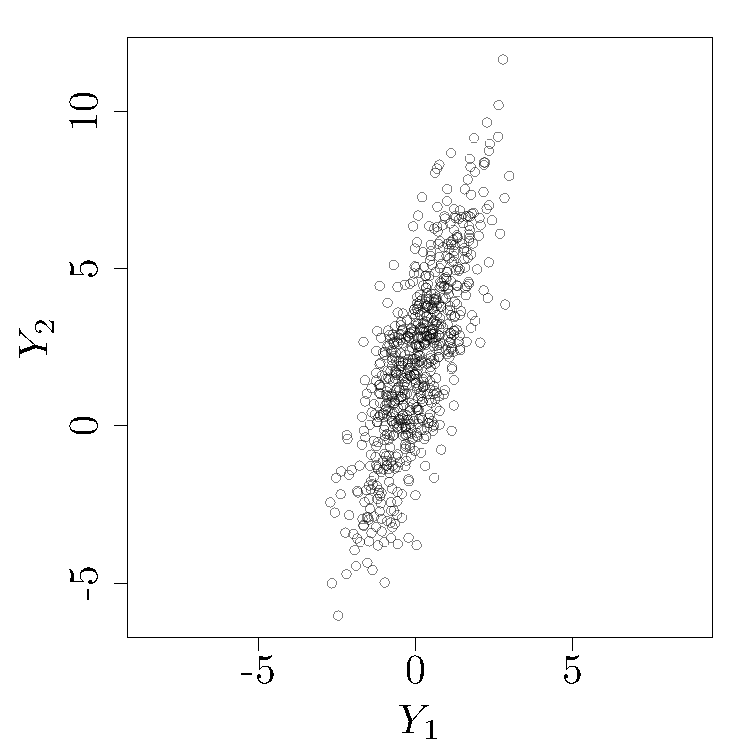
\includegraphics[width=\textwidth]{figures/ch1_gaussvec1}
                \caption{$\mu = (0,2),\ \Sigma= \left(\begin{smallmatrix} 1&2\\2&7 \end{smallmatrix} \right) $}
        \end{subfigure}%
        \hspace{1cm}       
        \begin{subfigure}[b]{0.34\textwidth}
                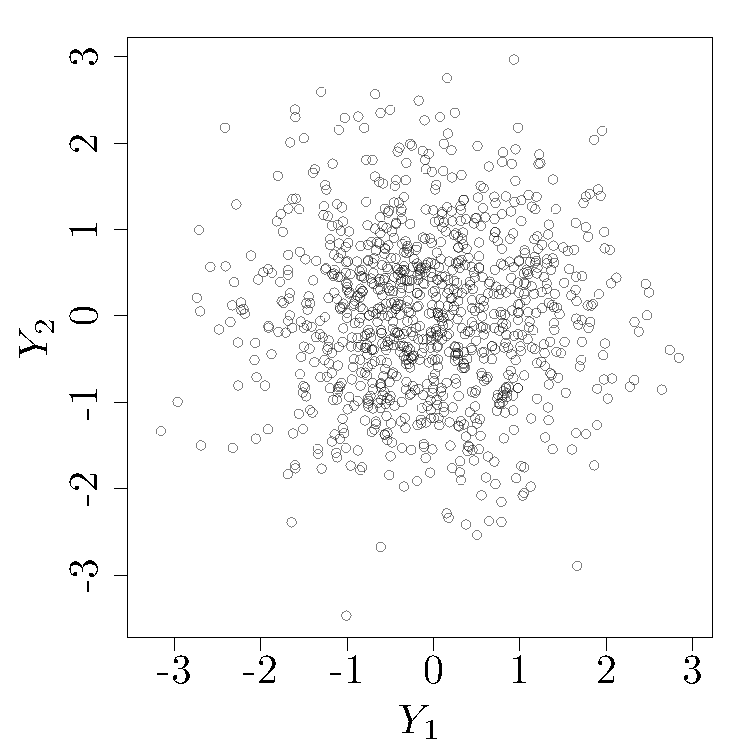
\includegraphics[width=\textwidth]{figures/ch1_gaussvec2}
                \caption{$\mu = (0,0),\ \Sigma= \left(\begin{smallmatrix} 1&0\\0&1 \end{smallmatrix} \right) $}
        \end{subfigure}
        \begin{subfigure}[b]{0.34\textwidth}
                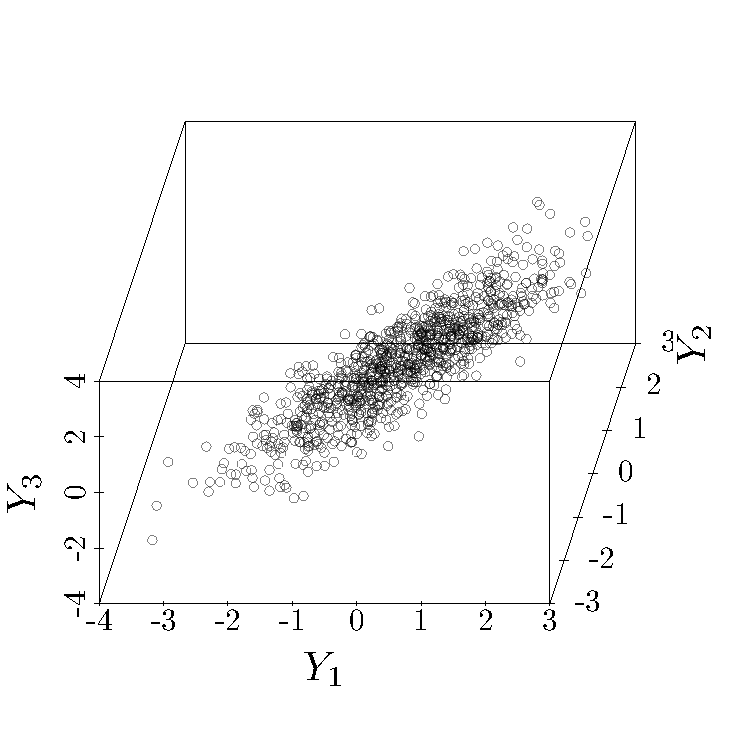
\includegraphics[width=\textwidth]{figures/ch1_gaussvec3}
                \caption{$\mu = (0,0,0),\ \Sigma= \left(\begin{smallmatrix} 1&0.4&0.8 \\ 0.4&0.5&0.3 \\ 0.8 & 0.3 & 1 \end{smallmatrix} \right) $}
        \end{subfigure}%
        \hspace{1cm}       
        \begin{subfigure}[b]{0.34\textwidth}
                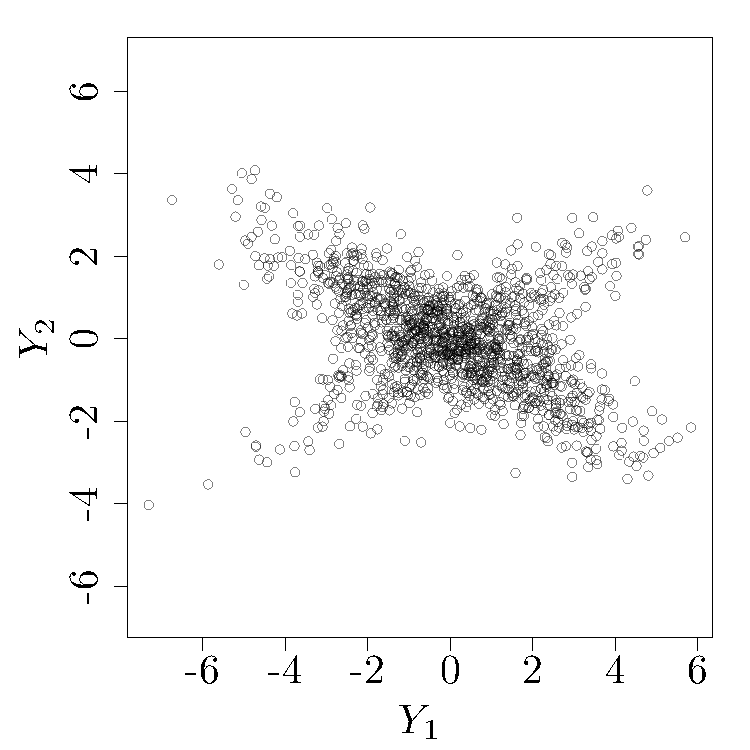
\includegraphics[width=\textwidth]{figures/ch1_gaussvec4}
                \caption{Non Gaussian samples}
        \end{subfigure}%
        \caption{The first three panels show samples from Gaussian vectors. Panel (d) shows samples from a random vector where each component is a Gaussian random variable (i.e.\@ the projection of the points on each axis is Gaussian) but the couple $(Y_1,Y_2)$ is not multivariate Gaussian (for example, the projection on one diagonal is not Gaussian).}
        \label{fig:vecsample}
\end{figure}

\paragraph{}
The probability density function of a multivariate normal random vector writes:
\begin{equation}
f_Y(x) = \frac{1}{\displaystyle | 2 \pi \Sigma|^{1/2}} \exp \left(-\frac12 (x-\mu)^t \Sigma^{-1} (x-\mu)  \right).
\label{eq:pdf}
\end{equation}  
where $\mu$ is the $d$-dimensional mean vector $\mu_i = \E[Y_i]$, and where $\Sigma$ is the $d \times d$ covariance matrix: $\Sigma_{i,j}=\Cov(Y_i, Y_j)$. In this expression, $| 2 \pi \Sigma|$ denotes the determinant of the matrix $2 \pi \Sigma$, which is thus equal to $(2 \pi)^d|  \Sigma|$. An example of 2-dimensional Gaussian density is represented in Figure~\ref{fig:vecpdf}.

\begin{figure}[ht!]
        \centering
        \begin{subfigure}[b]{0.34\textwidth}
                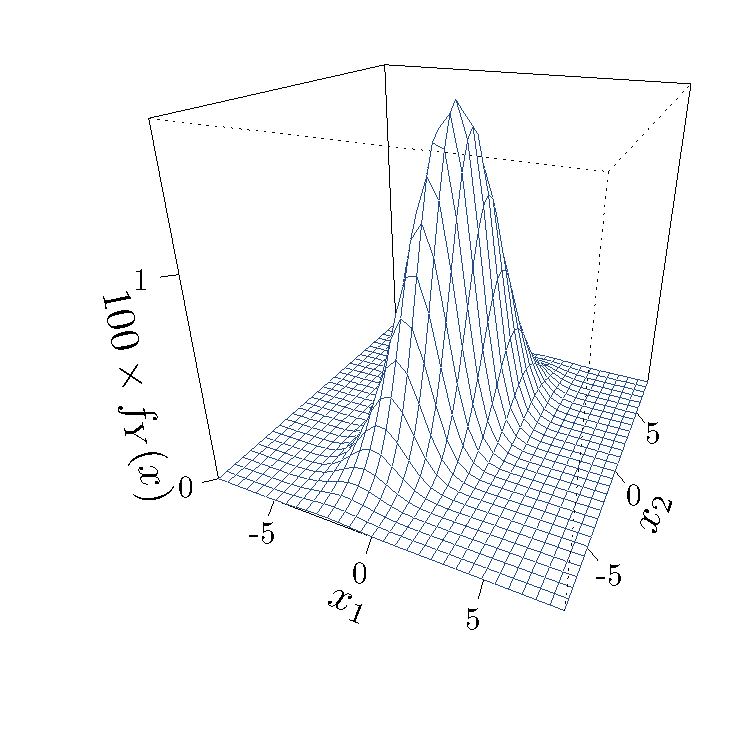
\includegraphics[width=\textwidth]{figures/ch1_pdf1}
                \caption{pdf shown as 3d-plot.}
        \end{subfigure}%
        \hspace{1cm}       
        \begin{subfigure}[b]{0.34\textwidth}
                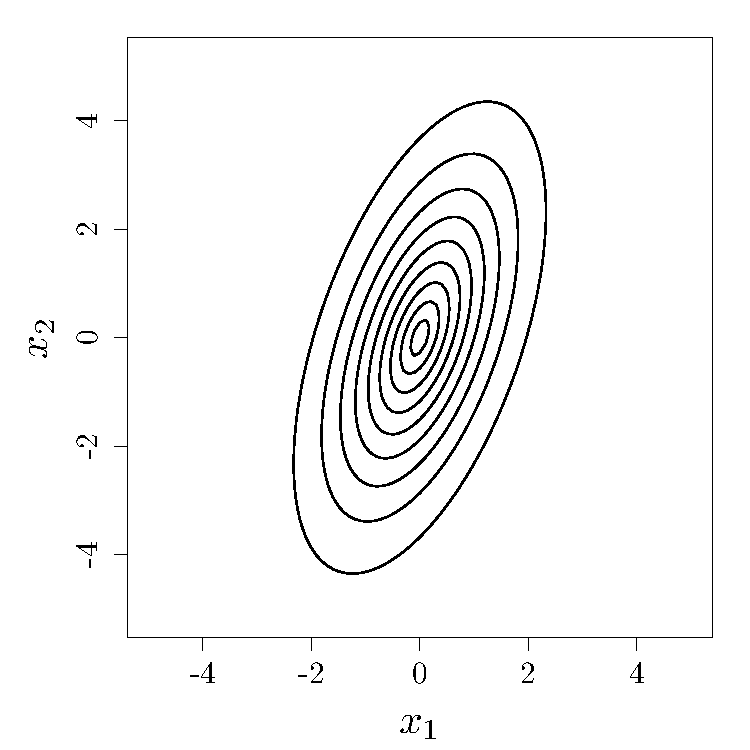
\includegraphics[width=\textwidth]{figures/ch1_pdf2}
                \caption{pdf shown as contour lines.}
        \end{subfigure}
        \caption[Example of multivariate Gaussian probability density function]{Example of multivariate Gaussian probability density function for $\mu = (0,0)^t$ and $\Sigma =  \left( \begin{smallmatrix} 2&2 \\ 2&7 \end{smallmatrix} \right)$. The level lines of Panel (b) are chosen such that the probability for a sample to be in any of the 10 regions delimited by the level lines is the same.}
        \label{fig:vecpdf}
\end{figure}

\paragraph{}
As can be seen in equation~\ref{eq:pdf}, the mean $\mu$ and the covariance matrix $\Sigma$ fully characterize a multivariate normal distribution. The distribution of a Gaussian random vector can thus be summarised by the notation $Y \sim \mathcal{N}(\mu,\Sigma)$. 

\paragraph{}
A covariance matrix has two important properties:
\begin{itemize}
 	\item It is symmetric: $\Sigma_{i,j} = \Cov(Y_i,Y_j) = \Cov(Y_j,Y_i) = \Sigma_{j,i}$
 	\item It is positive semi-definite: $\forall \alpha \in \mathds{R}^d,\ \alpha^t \Sigma \alpha = \Var(\alpha^t Y) \geq 0$.
 \end{itemize} 
Conversely, any matrix $K$ satisfying these two properties can be seen as a covariance matrix. Indeed, the symmetry of $K$ allows to diagonalize it in an orthonormal basis $K=PDP^t$ and its positive semi-definiteness ensure that all the diagonal elements of $D$ are non-negative. As a consequence, we can write $K=(PD^{1/2})(PD^{1/2})^t$ where $D^{1/2}$ is a diagonal matrix with entries $(D^{1/2})_{i,i}=\sqrt{D_{i,i}}$. Now, let $Z_1, \dots, Z_d$ be independent standard Gaussian random variables (i.e.\@ with zero mean and variance one) and let $Z=(Z_1, \dots, Z_d)^t$ be the associated Gaussian vector. It can the be shown that $K$ is the covariance matrix of $Y=PD^{1/2}Z$:
\begin{equation}
        \Var(Y) = \E[YY^t] - \underbrace{\E[Y]\E[Y^t]}_0 =  \E[PD^{1/2}Z Z^t(PD^{1/2})^t] = PD^{1/2} \underbrace{\E[Z Z^t]}_{I_d} (PD^{1/2})^t = K.
\end{equation}
This result is based on the property $PD^{1/2} (PD^{1/2})^t = K$, but $PD^{1/2}$ is not the only matrix $M$ satisfying $MM^t = K$. For example one can think about the Cholesky decomposition of $K$ which is less expensive to compute than an eigenvalue decomposition. Hereafter we will denote by $K^{1/2}$ any matrix that satisfy $K^{1/2} (K^{1/2})^t = K$. Whatever the choice of $K^{1/2}$, the proof above still apply and $Y=K^{1/2}Z$ will be $\mathcal{N}(0,K)$.

\paragraph{}
This scheme is of great interest to simulate Gaussian vector samples: if we want to obtain one sample from $Y \sim \mathcal{N}(\mu,\Sigma)$, the steps are:
\begin{enumerate}
        \item Compute $\Sigma^{1/2}$ (such as a Cholesky or $PD^{1/2}$).
        \item Generate a vector $Z = (Z_1, \dots, Z_d)^t$ of independent standard Gaussian samples.
        \item A sample of $Y$ is then given $\mu + \Sigma^{1/2}Z$.
\end{enumerate}

Although the independence of two variables always implies they are uncorrelated, one striking property of Gaussian vectors is that the converse is also true: 
\begin{property}
	For a Gaussian vector a correlation equal to zero implied independence.
\end{property}
\begin{proof}
	The covariance matrix of an uncorrelated Gaussian vector is a diagonal matrix which implies
\begin{equation}
f_Y(x) = \frac{1}{\displaystyle \sqrt{2 \pi \Sigma_{1,1}} \times \dots \times \sqrt{2 \pi \Sigma_{d,d}}} \exp \left(- \sum_{i=1}^d \frac{(x_i-\mu_i)^2 }{2\Sigma_{i,i}}  \right) = \prod_{i=1}^d f_{Y_i}(x_i).
\end{equation}
which is one of the definitions of independence.
\end{proof}

\subsection*{Conditional distribution of a Gaussian vector}
\label{sec:condvec}
Let $(Y_1,Y_2)$ be a Gaussian vector ($Y_1$ and $Y_2$ may both be vectors) with mean $\mu = (\mu_1,\mu_2)^t$ and covariance matrix
\begin{equation}
\Sigma = 
\begin{pmatrix}
	\Sigma_{1,1} & \Sigma_{1,2}\\
	\Sigma_{2,1} & \Sigma_{2,2}\\
\end{pmatrix}.
\end{equation}
\begin{property}
\label{prop:condGV}
The conditional distribution of $Y_1$ knowing $Y_2$ is still multivariate Gaussian:
\begin{equation}
\begin{split}
	Y_1|Y_2 \sim \mathcal{N}(\mu_c,\Sigma_c) \text{ with }\mu_c &= \E [Y_1|Y_2] = \mu_1 + \Sigma_{1,2} \Sigma_{22}^{-1} (Y_2-\mu_2)\\ 
	\Sigma_c &= \Cov [Y_1,Y_1|Y_2] = \Sigma_{1,1} - \Sigma_{1,2} \Sigma_{2,2}^{-1} \Sigma_{2,1},
\end{split}
\end{equation}
\end{property}
Before giving a formal proof, we give a graphical interpretation of this property in Figure~\ref{fig:condvecpdf}.
\begin{figure}[ht!]
        \centering
        \begin{subfigure}[b]{0.44\textwidth}
                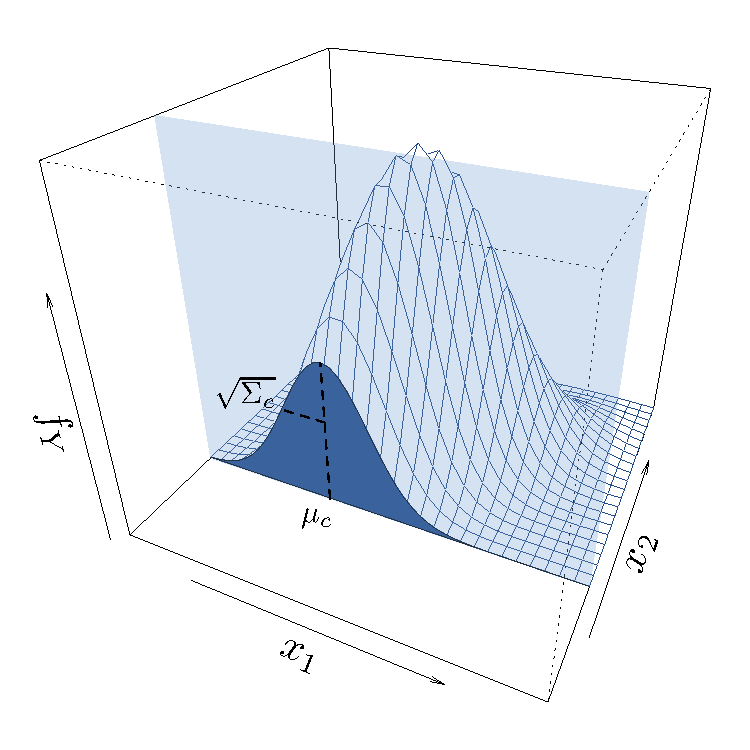
\includegraphics[width=\textwidth]{figures/ch1_condpdf1}
                \caption{2d example: density of $Y_1|Y_2 \shorteq -3.28$.}
        \end{subfigure}%
        \hspace{1cm}       
        \begin{subfigure}[b]{0.44\textwidth}
                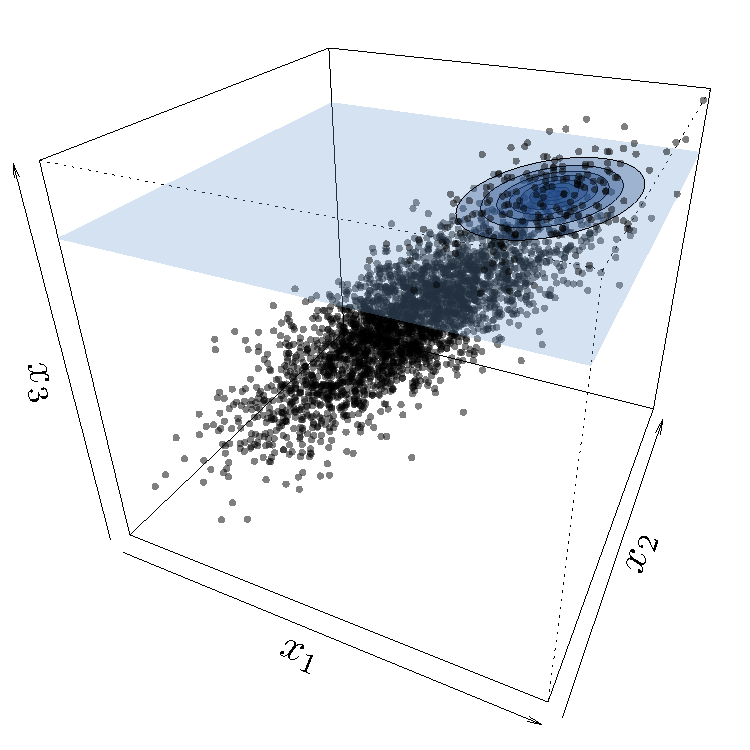
\includegraphics[width=\textwidth]{figures/ch1_condpdf2}
                \caption{3d example: density of $(Y_1,Y_2)|Y_3 \shorteq 2$.}
        \end{subfigure}
        \caption[Example of multivariate Gaussian probability density function]{Example of conditional multivariate Gaussian probability density functions.}
        \label{fig:condvecpdf}
\end{figure}

\begin{proof}
	Without loss of generality, we will assume that $(Y_1,Y_2)$ is centred. Up to the scaling factor ensuring the integral is equal to one, the density of this vector writes
	\begin{equation}
		f_{(Y_1,Y_2)}(x) \propto \exp \left( - (x_1^t\ x_2^t) 
		\begin{pmatrix}
			\Sigma_{1,1} & \Sigma_{1,2}\\
			\Sigma_{2,1} & \Sigma_{2,2}\\
		\end{pmatrix}^{-1}
		\begin{pmatrix}
			x_1\\
			x_2\\
		\end{pmatrix}
		 \right)
	\end{equation}
	The matrix block inverse formulae
	\begin{equation}
		\begin{pmatrix}
			A & B\\
			C & D\\
		\end{pmatrix}^{-1} = 
		\begin{pmatrix}
			(A-BD^{-1}C)^{-1} & -(A-BD^{-1}C)^{-1}BD^{-1}\\
			-D^{-1}C(A-BD^{-1}C)^{-1} & D^{-1} + D^{-1}C(A-BD^{-1}C)^{-1}BD^{-1}\\
		\end{pmatrix}
	\end{equation}	
	gives
	\begin{equation}
	\begin{split}
		f_{(Y_1,Y_2)}(x) \propto \exp  & \big(- x_1^t (\Sigma_{1,1}-\Sigma_{1,2}\Sigma_{2,2}^{-1}\Sigma_{2,1})^{-1} x_1 \\
		& + x_1^t (\Sigma_{1,1}-\Sigma_{1,2}\Sigma_{2,2}^{-1}\Sigma_{2,1})^{-1}\Sigma_{1,2}\Sigma_{2,2}^{-1} x_2 \\
		&+ x_2^t \Sigma_{2,2}^{-1}\Sigma_{2,1}(\Sigma_{1,1}-\Sigma_{1,2}\Sigma_{2,2}^{-1}\Sigma_{2,1})^{-1} x_1 \\
		&  - x_2^t (\Sigma_{2,2}^{-1} + \Sigma_{2,2}^{-1}\Sigma_{2,1}(\Sigma_{1,1}-\Sigma_{1,2}\Sigma_{2,2}^{-1}\Sigma_{2,1})^{-1}\Sigma_{1,2}\Sigma_{2,2}^{-1}) x_2 \big)
	\end{split}
	\end{equation}
Since we are interested in the distribution of $Y_1 | Y_2$, we can rearrange this expression to make it a quadratic form in $x_1$. Furthermore, we can consider that $x_2$ is fixed and we can include all the terms that do not depend in $x_1$ in the constant:
	\begin{equation}
	\begin{split}
		f_{(Y_1,Y_2)}(x) \propto \exp  & \big(- (x_1 - x_2^t \Sigma_{2,2}^{-1}\Sigma_{2,1})^t (\Sigma_{1,1}-\Sigma_{1,2}\Sigma_{2,2}^{-1}\Sigma_{2,1})^{-1} (x_1- \Sigma_{1,2}\Sigma_{2,2}^{-1} x_2) \big)\\
	\end{split}
	\end{equation}
As stated in the proposition, we recognize here the shape of the multivariate normal probability density function with mean $\Sigma_{1,2}\Sigma_{2,2}^{-1} x_2$ and variance $\Sigma_{1,1}-\Sigma_{1,2}\Sigma_{2,2}^{-1}\Sigma_{2,1}$.
\end{proof}

%%%%%%%%%%%%%%%%%%%%%%%%%%%%%%%%%%%%%%%%%%%%%%%
\section{Gaussian processes}

\paragraph{}
Multivariate random variables can be generalised to \emph{random processes}, which are also called \emph{stochastic processes}. In this case, each draw returns a function. There are many different types of random processes (Poisson processes, Levy processes, etc.) and we will focus hereafter on Gaussian processes which generalize the multivariate normal distribution.

\begin{definition}
A random process $Z$ over a domain $D \subset \mathds{R}^d$ is said to be Gaussian if 
\begin{equation}
\forall n \in \mathds{N}, \forall x_i \in D, (Z(x_1),\dots,Z(x_n)) \text{  is a Gaussian vector}.
\end{equation} 
\end{definition}
The distribution of a Gaussian process is fully characterised by its mean function defined over $D$: $m(x)= \E[Z(x)]$ and its covariance function (or kernel) $k$ defined over $D \times D$: $k(x,y) = \Cov(Z(x),Z(y))$. As previously, we use the notation $Z \sim \mathcal{N}(m(.),k(.,.))$. Examples of Gaussian process sample path are given in Figure~\ref{fig:GPsample}.

\begin{figure}
        \centering
        \begin{subfigure}[t]{0.34\textwidth}
                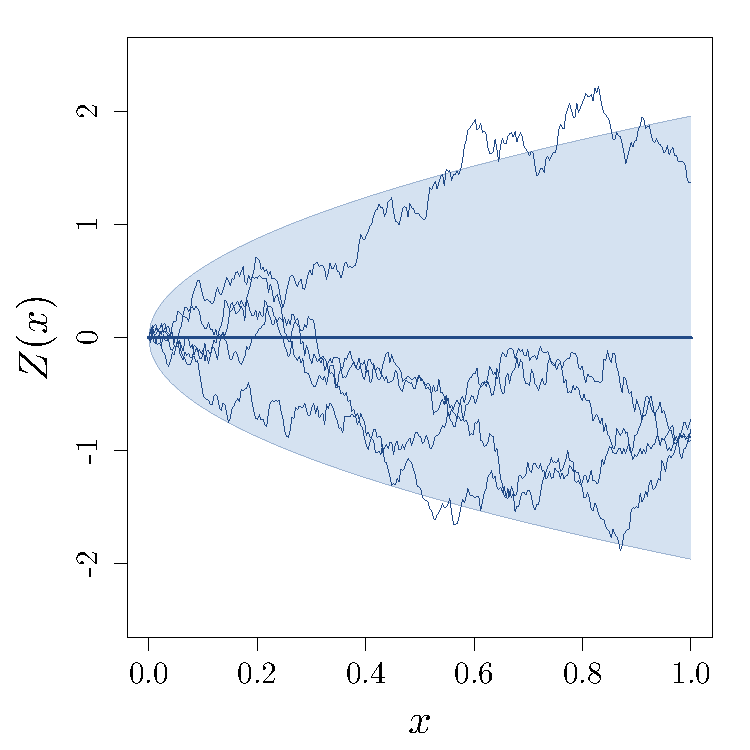
\includegraphics[width=\textwidth]{figures/ch1_GPpath0}
                \caption{Brownian motion: \\$m(x) = 0,\ k(x,y)= \min(x,y)$}
        \end{subfigure}%
        \hspace{1cm}       
        \begin{subfigure}[t]{0.34\textwidth}
                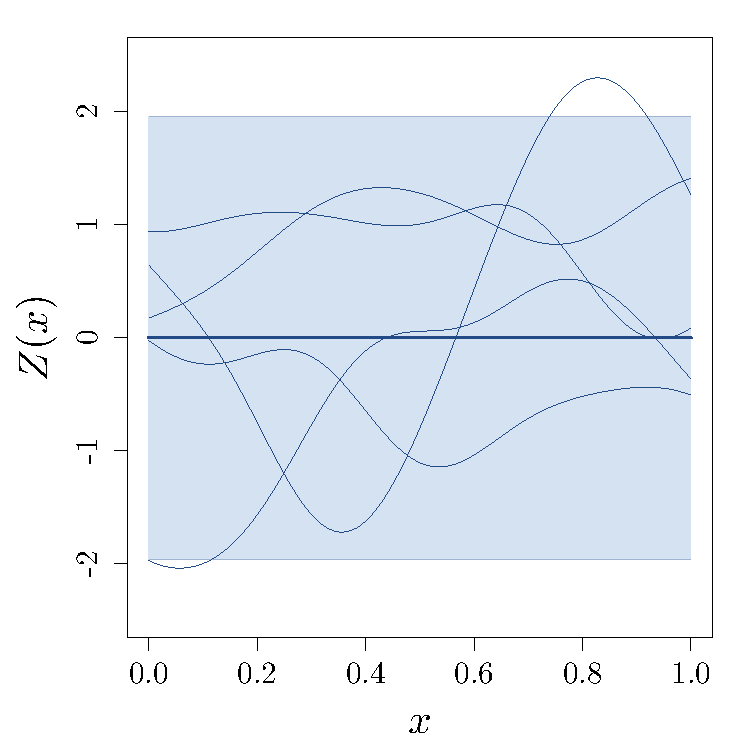
\includegraphics[width=\textwidth]{figures/ch1_GPpath2}
                \caption{$m(x) = 0$ and Gaussian covariance}
                \label{fig:GPsampleb}
        \end{subfigure}
        \begin{subfigure}[t]{0.34\textwidth}
                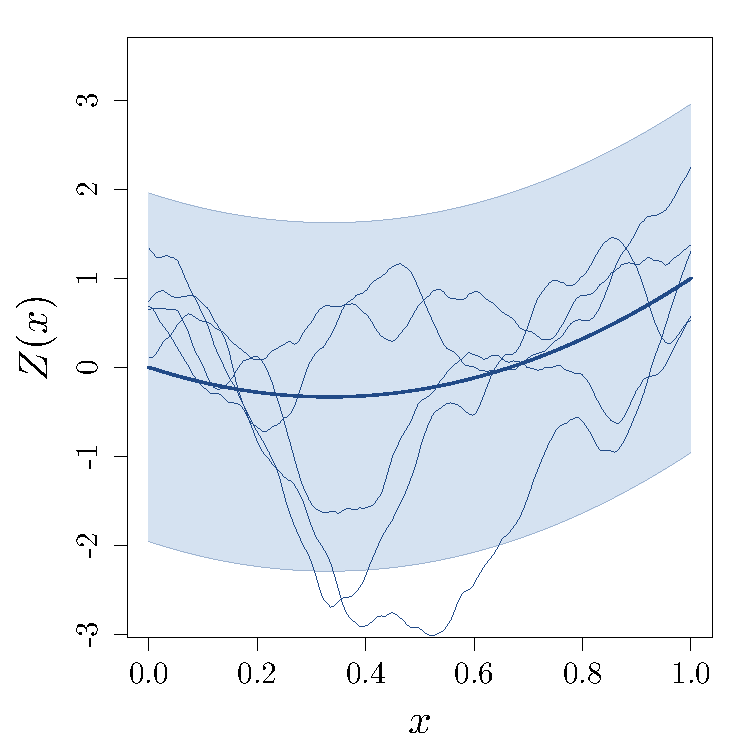
\includegraphics[width=\textwidth]{figures/ch1_GPpath3}
                \caption{$m(x) = -2x + 3x^2$ and Mat\'ern 3/2 covariance}
        \end{subfigure}%
        \hspace{1cm}       
        \begin{subfigure}[t]{0.34\textwidth}
                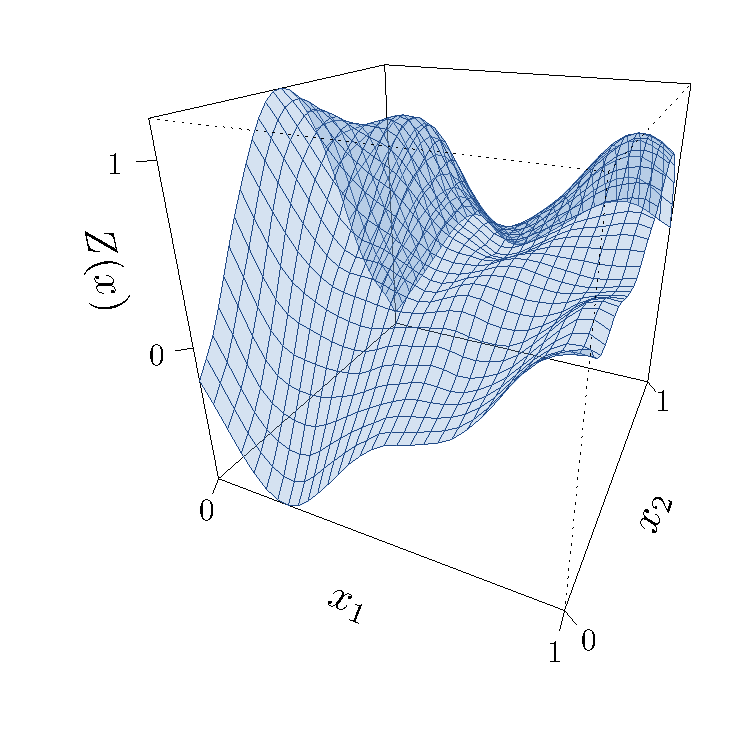
\includegraphics[width=\textwidth]{figures/ch1_GPpath4}
                \caption{$m(x) = 0$ and Mat\'ern 5/2 covariance}
        \end{subfigure}%
        \caption{Examples of sample paths of Gaussian processes for various means and covariance functions. For the first three panels, the thick line shows the mean function $m$ and the shaded area corresponds to 95\% confidence intervals. For the 2D example (last panel), only one sample is shown. The method for obtaining such sample paths is to consider the value of the process on a fine grid $(Z(x_1), \dots,Z(x_{100}))$ and then to use the method presented above for sampling this Gaussian vector.}
        \label{fig:GPsample}
\end{figure}

\paragraph{}
We have seen previously that a covariance matrix is positive semi-definite. This notion can be generalised to functions: 
\begin{definition}
\label{def:pdf}
	A function $k(.,.)$ over $D \times D$ is positive semi-definite if is satisfies
	\begin{equation*}
		\forall n \in \mathds{N}, \forall \{x_1,\dots,x_n\} \in D^n, \forall \alpha \in \mathds{R}^n,\  \sum_{i=1}^n \sum_{j=1}^n \alpha_i \alpha_j k(x_i,x_j) \geq 0.
	\end{equation*}
	In other words, $\forall n \in \mathds{N}, \forall x_i \in D$, the $n \times n$ matrix of general term $K_{i,j} = k(x_i,x_j)$ is positive semi-definite.
\end{definition}
The equivalence between symmetric positive semi-definite functions and covariance function is given by the following theorem:
\begin{theorem}[Loeve]
\label{thm:loeve}
	A covariance function is symmetric positive semi-definite and any symmetric positive semi-definite function can be seen as a covariance function. 
\end{theorem}

\section{Covariance functions}
\label{sec:kernels}
As can be seen from Definition~\ref{def:pdf}, showing that a function is positive semi-definite directly from the definition is intractable since the inequality has to be proven $\forall n \in \mathds{N}, \forall x_i \in D$ and $\forall \alpha \in \mathds{R}^n$. In practice, there is a very wide variety of covariance functions that have been proven to be positive definite and one can use any one of them as a Gaussian process covariance.

\paragraph{} 
Before giving a list of the most common covariances, we will notice that if $Z$ is a Gaussian process with covariance $k$, then a rescaling of the horizontal and vertical axis by two parameters $\theta$ and $\sigma$ allows to define a new Gaussian process $\tilde{Z}(x) = \sigma Z(x/\theta)$. Direct calculation shows that the covariance of $\tilde{Z}$ is $\sigma^2 k(x/\theta,y/\theta)$. $\sigma^2$ can then be interpreted as a variance parameter and $\theta$  will be called the length scale parameter. These parameters are usually included in the kernels definitions.

\paragraph{} 
The most common one-dimensional and $d$-dimensional covariances are regrouped in Tables~\ref{tab:ker1d} and~\ref{tab:kerdimd}. One can notice that many covariances in these tables depends on $x$ and $y$ only by the difference $x-y$, which implies that the distribution of the process does not change when we translate the input space. Such covariances are called \emph{stationary covariances} and they are often written as a function of one variable: $k(x-y)$.
\begin{table}[b]
\begin{center}
\begin{tabular}{|rlN|}
		\hline
		Name & Expression &\\[4mm]  \hline 
		squared exponential$^1$ & $\displaystyle k(x,y) = \sigma^2 \exp \left(- \frac{(x-y)^2}{2 \theta^2} \right)$ &\\[6mm]
		Matern 5/2 & $\displaystyle k(x,y) = \sigma^2 \left(1 + \frac{\sqrt{5}|x-y|}{\theta} + \frac{5|x-y|^2}{3 \theta^2} \right) \exp \left(- \frac{\sqrt{5}|x-y|}{\theta} \right)$ &\\[6mm]
		Matern 3/2 & $\displaystyle k(x,y) = \sigma^2 \left(1 + \frac{\sqrt{3}|x-y|}{\theta} \right) \exp \left(- \frac{\sqrt{3}|x-y|}{\theta} \right)$ &\\[6mm]
		exponential & $\displaystyle k(x,y) = \sigma^2 \exp \left(- \frac{|x-y|}{\theta} \right)$ &\\[6mm]
		Brownian\footnote{Only defined over $\mathds{R}^{+} \times \mathds{R}^+$} & $ \displaystyle k(x,y) = \sigma^2 \min (x,y) $ &\\[6mm]
		white noise & $ \displaystyle k(x,y) = \sigma^2 \delta_{x,y} $ &\\[6mm]
		constant & $ \displaystyle k(x,y) = \sigma^2 $ &\\[6mm]
		linear & $ \displaystyle k(x,y) = \sigma^2 xy $ &\\[6mm]
		cosine & $ \displaystyle k(x,y) = \sigma^2 \cos \left (\frac{x-y}{\theta} \right) $ &\\[6mm]
		sinc & $ \displaystyle k(x,y) = \sigma^2 \frac{\theta}{x-y} \sin \left( \frac{x-y}{\theta} \right) $ &\\[6mm] \hline
\end{tabular}
\end{center}
\hspace{1cm} \footnotesize{$^1$ Also called Gaussian kernel, radial basis function (rbf) or exponentiated quadratic.}
\caption{Examples of (common) one-dimensional kernels.}
\label{tab:ker1d}
\end{table}

\paragraph{}
If we want to generalise these expressions for $d$-dimensional input spaces, we might want to introduce one rescaling parameter per dimension. The usual Euclidean distance between two points $|| x-y || = ( \sum (x_i-y_i)^2)^{1/2}$ is thus replaced by
\begin{equation}
	\N{x-y}{\theta} = \left( \sum_{i=1}^d \frac{(x_i-y_i)^2}{\theta_i^2} \right)^{1/2}.
\end{equation}
If the parameters $\theta_i$ are equal for all dimensions, the covariance (or the process) is called isotropic. The covariances of Table~\ref{tab:ker1d} that can be generalised in higher dimension are given in Table~\ref{tab:kerdimd}.  
\begin{table}
\begin{center}
\begin{tabular}{|rlN|}
        \hline
        Name & Expression &\\[4mm]  \hline 
        squared exponential$^1$ & $\displaystyle k(x,y) = \sigma^2 \exp \left(- \frac12 \N{x-y}{\theta}^2 \right)$ &\\[6mm]
        Mat\'ern 5/2 & $\displaystyle k(x,y) = \sigma^2 \left(1 + \sqrt{5}\N{x-y}{\theta} + \frac{5}{3}\N{x-y}{\theta}^2 \right) \exp \left(- \sqrt{5}\N{x-y}{\theta} \right)$ &\\[6mm]
        Mat\'ern 3/2 & $\displaystyle k(x,y) = \sigma^2 \left(1 + \sqrt{3}\N{x-y}{\theta} \right) \exp \left(- \sqrt{3}\N{x-y}{\theta}  \right)$ &\\[6mm]
        exponential & $\displaystyle k(x,y) = \sigma^2 \exp \left(- \N{x-y}{\theta} \right)$ &\\[6mm]
        white noise & $ \displaystyle k(x,y) = \sigma^2 \delta_{x,y} $ &\\[6mm]
        constant & $ \displaystyle k(x,y) = \sigma^2 $ &\\[6mm]
        linear & $ \displaystyle k(x,y) = \sum_{i=1}^d \sigma^2_i x_iy_i $ &\\[6mm]
        % cosine & $ \displaystyle k(x,y) = \sigma^2 \cos \left ( \N{x-y}{\theta} \right) $ &\\[6mm]
        % sinc & $ \displaystyle k(x,y) = \sigma^2 \frac{1}{\N{x-y}{\theta}} \sin \left( \N{x-y}{\theta} \right) $ &\\[6mm]     
        \hline
\end{tabular}
\end{center}
\hspace{1cm} \footnotesize{$^1$ Also called Gaussian kernel, radial basis function (rbf) or exponentiated quadratic.}
\caption{Examples of common $d$-dimensional kernels.}
\label{tab:kerdimd}
\end{table}

%%%%%%%%%%%%%%%%%%%%%%%%%%%%%%%%%%%%%%%%%%%%%%%%%%%%%%%%%%%%
%%%%%%%%%%%%%%%%%%%%%%%%%%%%%%%%%%%%%%%%%%%%%%%%%%%%%%%%%%%%
\chapter{Gaussian process regression}
In this section, we will detail how to approximate a function $f:\ D \subset \mathds{R}^d \rightarrow  \mathds{R}$ based on $n$ evaluations of the function. The set of points where the function is evaluated is called the design of experiments and it is represented by a $n \times d$ matrix $X$. The observations will be denoted by a column vector $F = f(X)$.  

\section{Interpolation}
% observations are not sufficient -> need to add information (for example choose a space). Assumption in GPR, f is a sample path of a GP Z.
The principle of Gaussian process regression is to combine a prior belief on the function we want to approximate and some actual observations of the function. From a mathematical point of view, the prior belief is given by a Gaussian process which can be seen as a distribution over functions. This framework allows to specify a very wide variety of prior beliefs such as the regularity of the function to approximate, its stationarity, periodicity, etc. but some other types of information such as the positivity or monotony cannot be encapsulated in Gaussian process priors.

\paragraph{}
Let $Z$ be a Gaussian process over $D$. We will assume that it is zero-mean with kernel $k$. The approximation of $f$ based on the prior $Z$ and the observations $F = f(X)$ is given by the conditional distribution of $Z$ knowing that it interpolates the data points. According to the definition of a Gaussian process, $(Z(x),Z(y),Z(X))$ is multivariate normal so Property~\ref{prop:condGV} applies and reads:
\begin{equation}
	\begin{split}
		m(x) &= \E[Z(x)|Z(X) \shorteq F] = k(x,X) k(X,X)^{-1} F\\
		c(x,y) &=  \Cov[Z(x),Z(y)|Z(X) \shorteq F] = k(x,y) - k(x,X) k(X,X)^{-1} k(X,y)
	\end{split}
	\label{eq:GPR}
\end{equation}
Figure~\ref{fig:GPR} shows one example of Gaussian process regression model.

\begin{figure}[ht!]
        \centering
        \begin{subfigure}[t]{0.3\textwidth}
                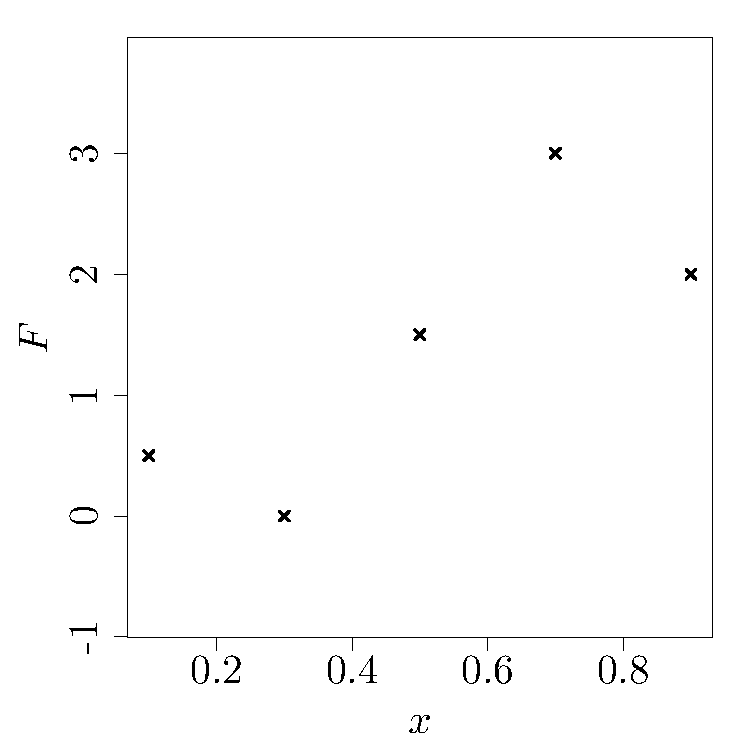
\includegraphics[width=\textwidth]{figures/ch2_obs}
                \caption{Observations}
        \end{subfigure}%
        ~         
        \begin{subfigure}[t]{0.3\textwidth}
                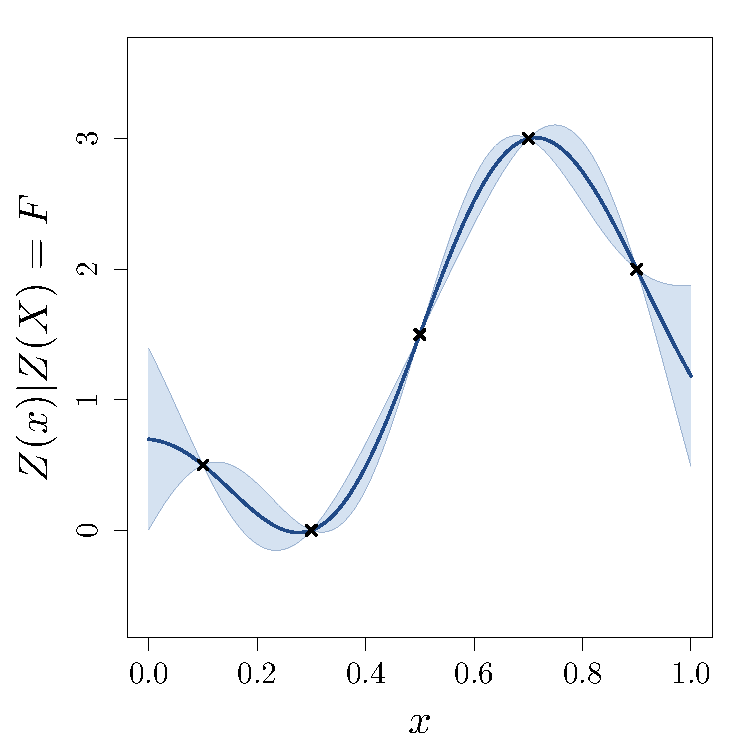
\includegraphics[width=\textwidth]{figures/ch2_GPR}
                \caption{mean predictor and 95\% confidence intervals}
        \end{subfigure}%
        ~ 
        \begin{subfigure}[t]{0.3\textwidth}
                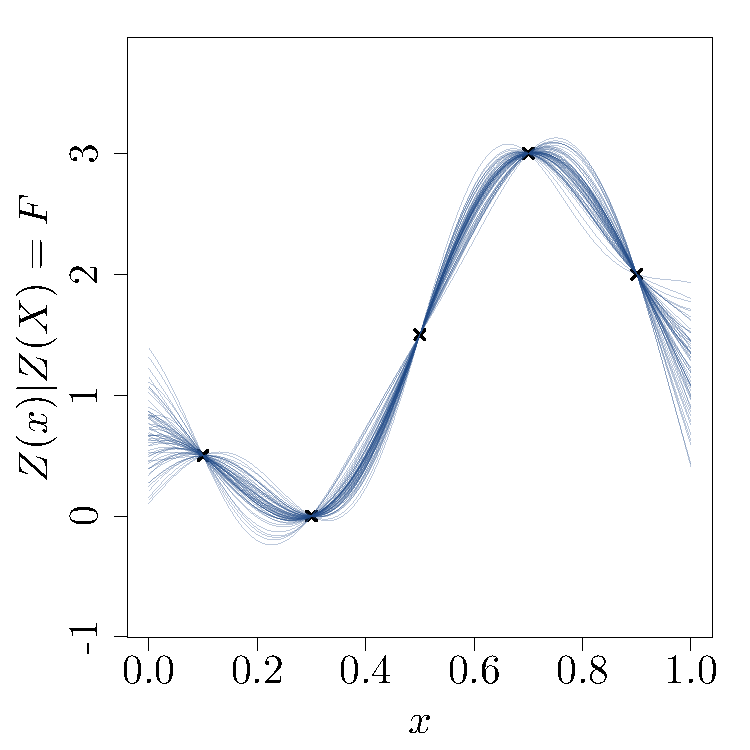
\includegraphics[width=\textwidth]{figures/ch2_GPcond}
                \caption{Conditional paths}
        \end{subfigure}%
        \caption{Example of Gaussian process regression model. On panel (b), the 95\% confidence intervals are given by $m(x) \pm 1.96\sqrt{c(x,x)}$. The prior $Z$ is the same as in Figure~\ref{fig:GPsampleb}.}
        \label{fig:GPR}
\end{figure}

\paragraph{}
We will now discuss a few properties of Gaussian process regression models: 
\begin{itemize}
	\item $m$ interpolates the data points. This can be explained either by 
	\begin{itemize}
	 	\item the properties of a conditional expectation: $m(X)=\E[Z(X)|Z(X) \shorteq F]=F$
	 	\item linear algebra: $m(X)=k(X,X) k(X,X)^{-1} F=F$
	 \end{itemize}
	\item The conditional variance $v(x) = c(x,x)$ is equal to zero at the observation points. The explanation is similar to the previous bullet point. 
	\item The conditional covariance does not depends on the observations $F$
	\item The best predictor can be seen either as a linear combination of the observations ($m(x)=\alpha^t F$) or as a linear combination of the kernel evaluated at the design of experiments ($m(x)=k(x,X) \beta$). The latter gives an insight on the model behaviour. For example
	\begin{itemize}
	 	\item The mean predictor of a model based on a Brownian kernel will be linear per block since it is a linear combination of $min(x,X)$ (see Figure~\ref{fig:GPRbasisfunctions})
	 	\item A model based on a stationary kernel such as a squared exponential kernel or a kernel from the Mat\'ern family will tend towards 0 (or the process mean if it is not centred) when the prediction point is far from the observations (see Figure~\ref{fig:GPRbasisfunctions}).
	 \end{itemize} 
\end{itemize}

\begin{figure}
        \centering
        \begin{subfigure}[t]{0.45\textwidth}
                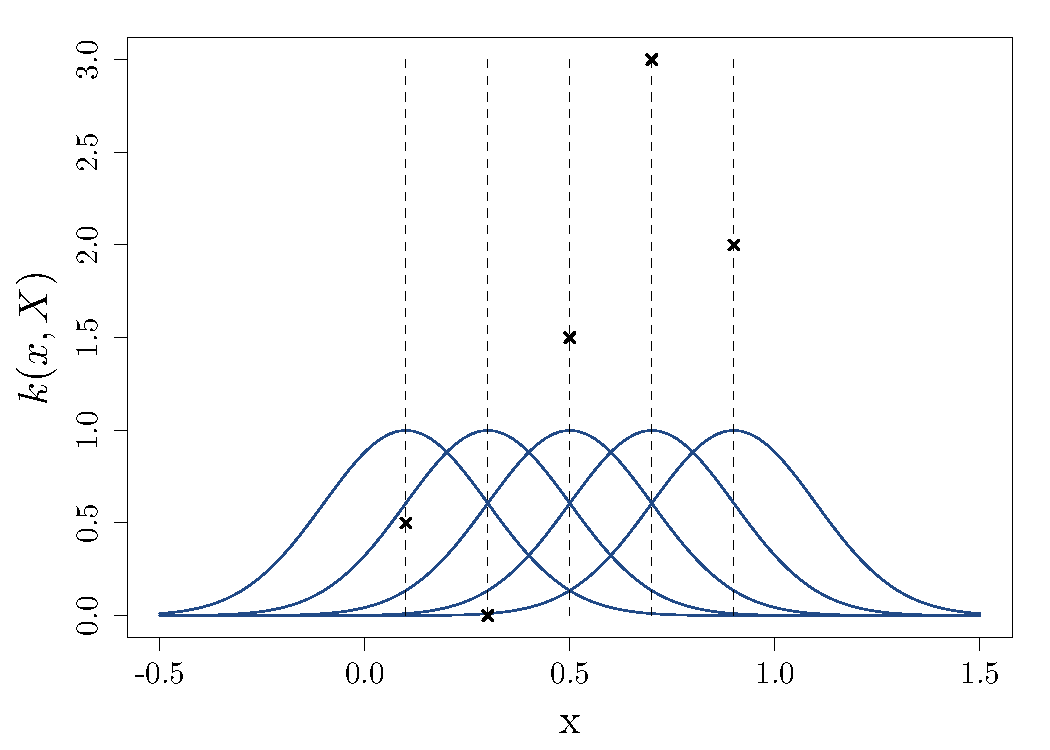
\includegraphics[width=\textwidth]{figures/ch2_basisfuncGauss}
                \caption{Basis functions: $\exp(-(x-X_i)^2/0.08)$.}
        \end{subfigure}%
        ~         
        \begin{subfigure}[t]{0.45\textwidth}
                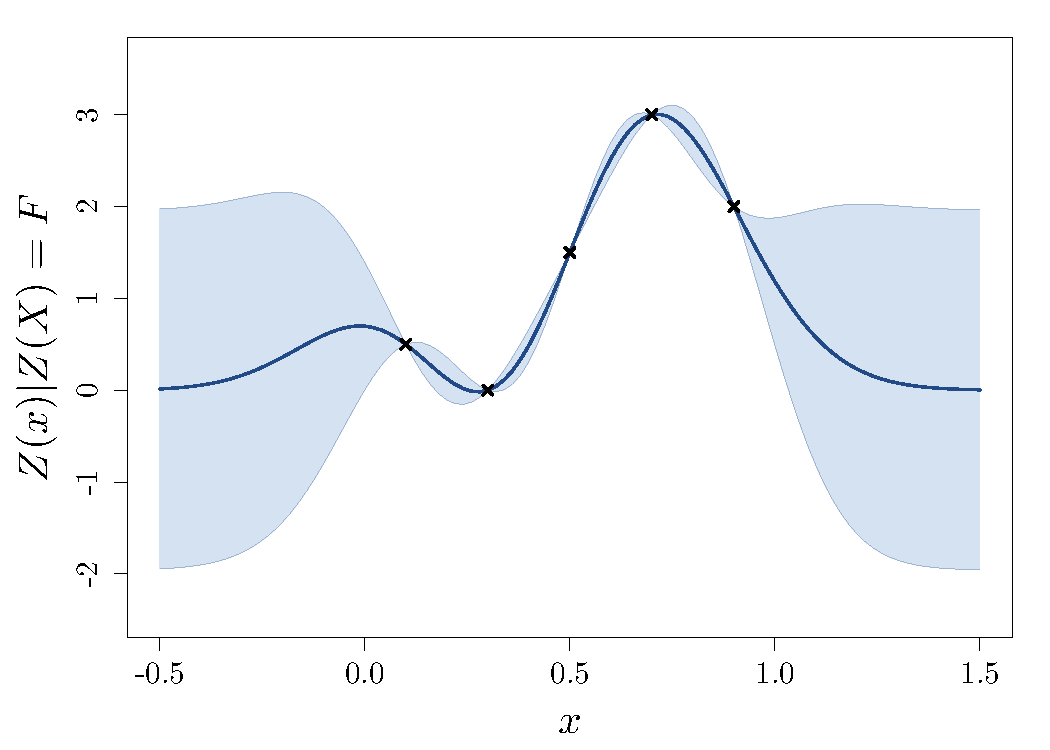
\includegraphics[width=\textwidth]{figures/ch2_GPRbasisfuncGauss}
                \caption{GPR model.}
        \end{subfigure}%
        \\
        \begin{subfigure}[t]{0.45\textwidth}
                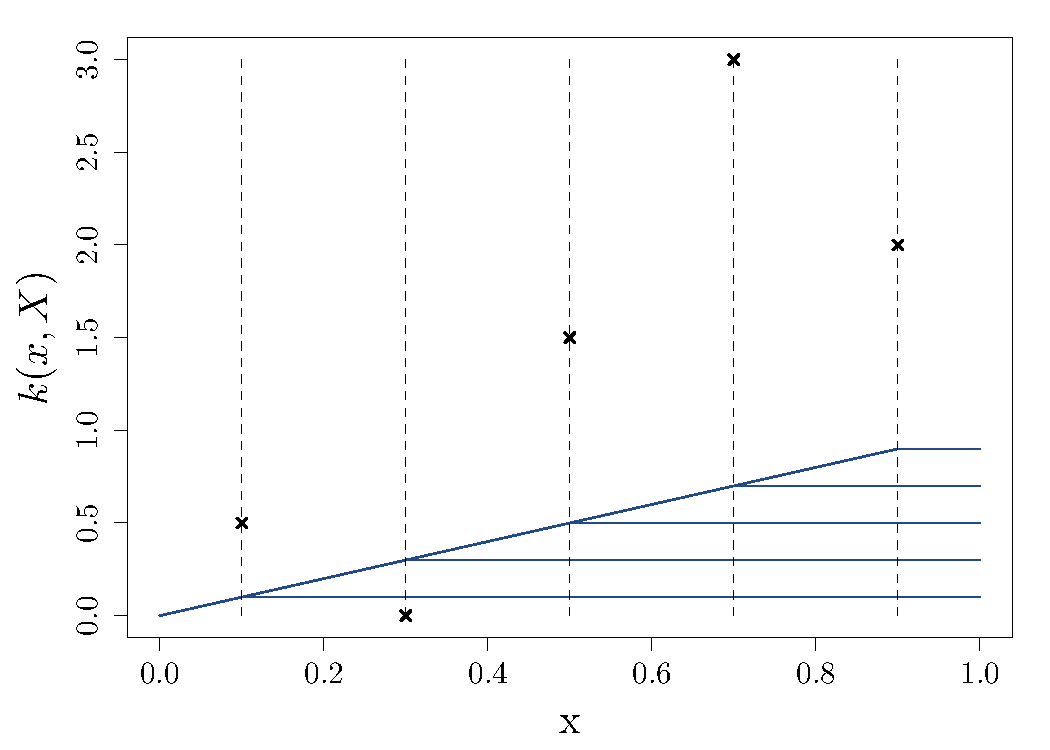
\includegraphics[width=\textwidth]{figures/ch2_basisfuncBrown}
                \caption{basis functions: $\min(x,X_i)$.}
        \end{subfigure}%
        ~
        \begin{subfigure}[t]{0.45\textwidth}
                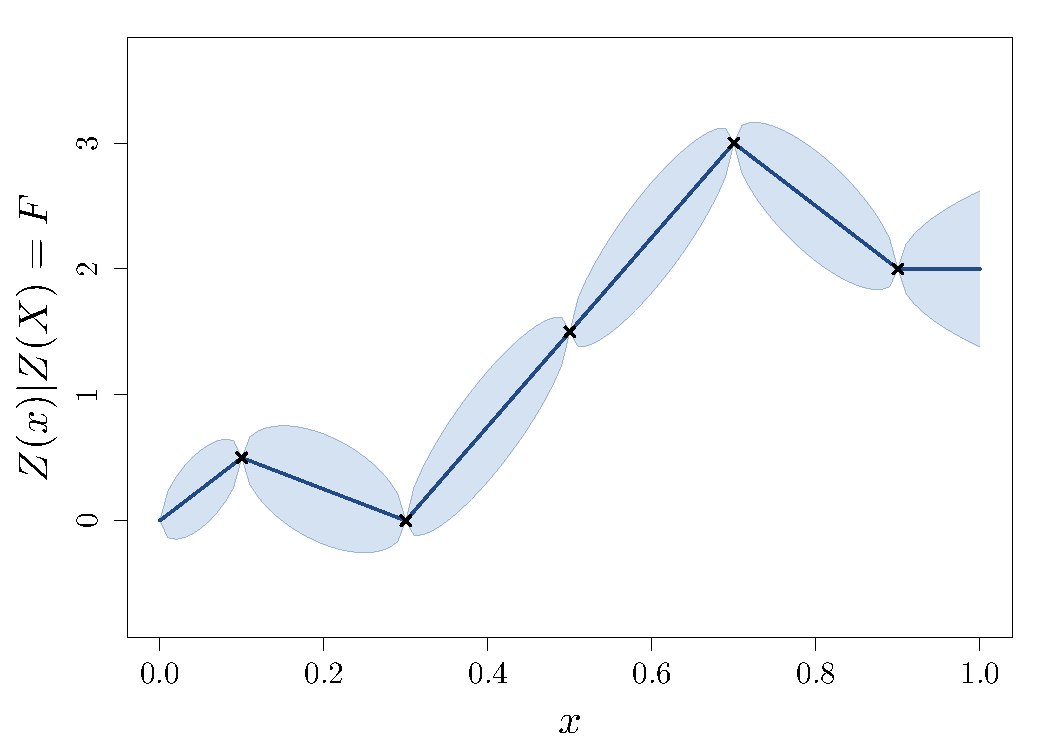
\includegraphics[width=\textwidth]{figures/ch2_GPRbasisfuncBrown}
                \caption{GPR model.}
        \end{subfigure}%
        \caption{Examples of Gaussian process regression model and their associated basis functions. The top panels are for a Gaussian kernel with parameters $(\sigma^2,\theta^2)=(1,0.2)$, and the lower ones are for a Brownian kernel with variance $\sigma^2 = 1$. }
        \label{fig:GPRbasisfunctions}
\end{figure}

\section{Approximation}
\paragraph{}
Interpolating the observations is not always a desirable feature. For example, when the observations are corrupted by some observation noise, it is preferable to have a model that smooths the observations instead of interpolating them. This approximation approach is called regularisation. 

\paragraph{}
The method for building a regularisation model is exactly the same as previously, but instead of assuming that the observations are given by the evaluation of a process $Z(X)=F$, we include a centred Gaussian process $N$ with kernel $n(.,.)$ that accounts for the observation noise in the model. According to this model, the signal is corrupted by $N(X)$ at observation points: $Z(X)+N(X)=F$. The Gaussian process regression equations then become:
\begin{equation}
	\begin{split}
		m(x) &= \E[Z(x)|Z(X)+N(X) \shorteq F] = k(x,X) (k(X,X)+n(X,X))^{-1} F\\
		c(x,y) &=  \Cov[Z(x),Z(y)|Z(X)+N(X) \shorteq F] = k(x,y) - k(x,X) (k(X,X)+n(X,X))^{-1} k(X,y)
	\end{split}
	\label{eq:noisyGPR}
\end{equation}
If observation noise can be described by independent $\mathcal{N}(0,\tau^2)$ variables, which is the most common case, the covariance matrix $n(X,X)$ is equal to $\tau^2$ times the identity matrix. Figure~\ref{fig:GPRnoise} shows the influence of this parameter on a toy example. It can be seen from this figure that $m$ does not interpolates the data points any more. Indeed, when we compute $m(X)$, we do not recognise the product of one matrix times its inverse as previously. Similarly, the prediction variance is not zero at the observation points.

\begin{figure}
        \centering
        \begin{subfigure}[t]{0.3\textwidth}
                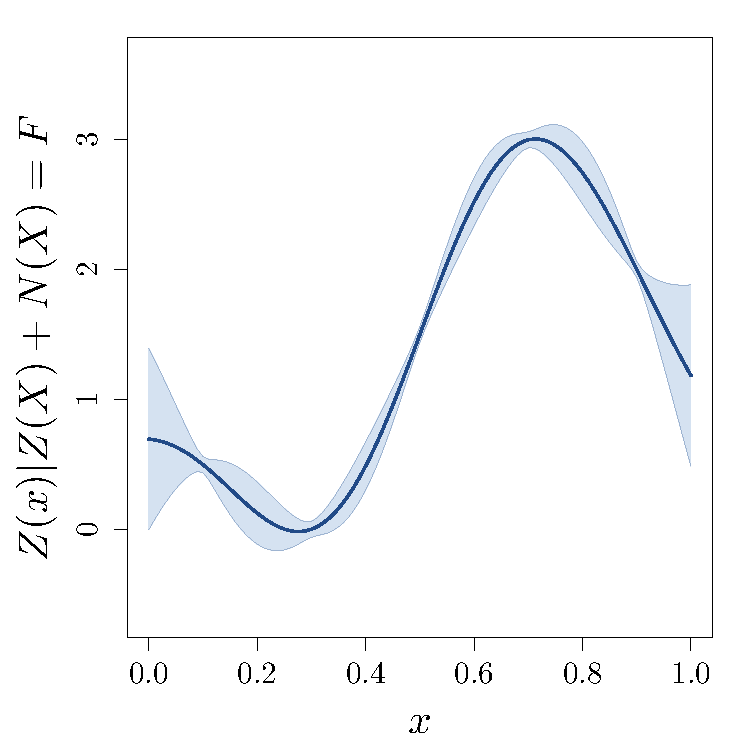
\includegraphics[width=\textwidth]{figures/ch2_GPRnoise0001}
                \caption{$\tau^2 = 0.001$}
        \end{subfigure}%
        ~         
        \begin{subfigure}[t]{0.3\textwidth}
                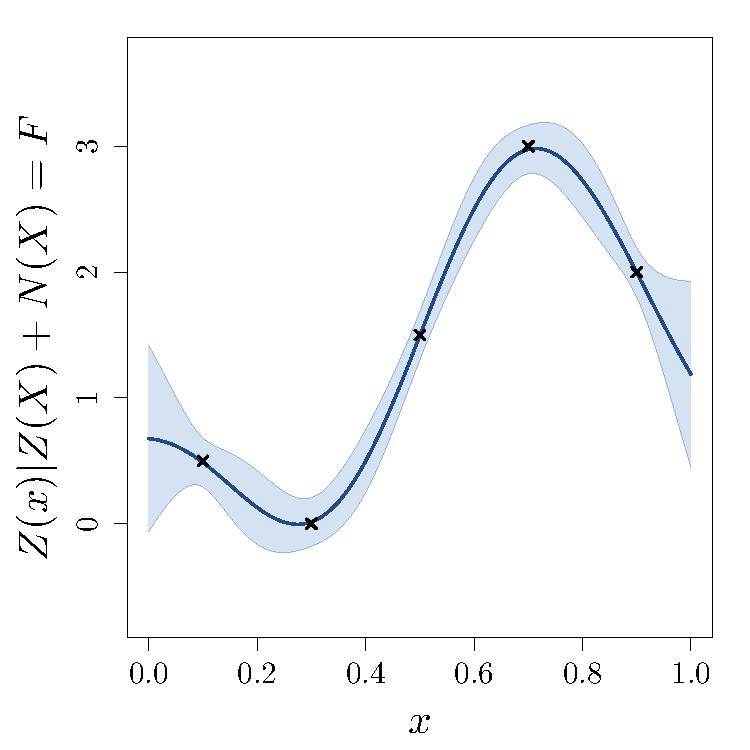
\includegraphics[width=\textwidth]{figures/ch2_GPRnoise001}
                \caption{$\tau^2 = 0.01$}
        \end{subfigure}%
        ~ 
        \begin{subfigure}[t]{0.3\textwidth}
                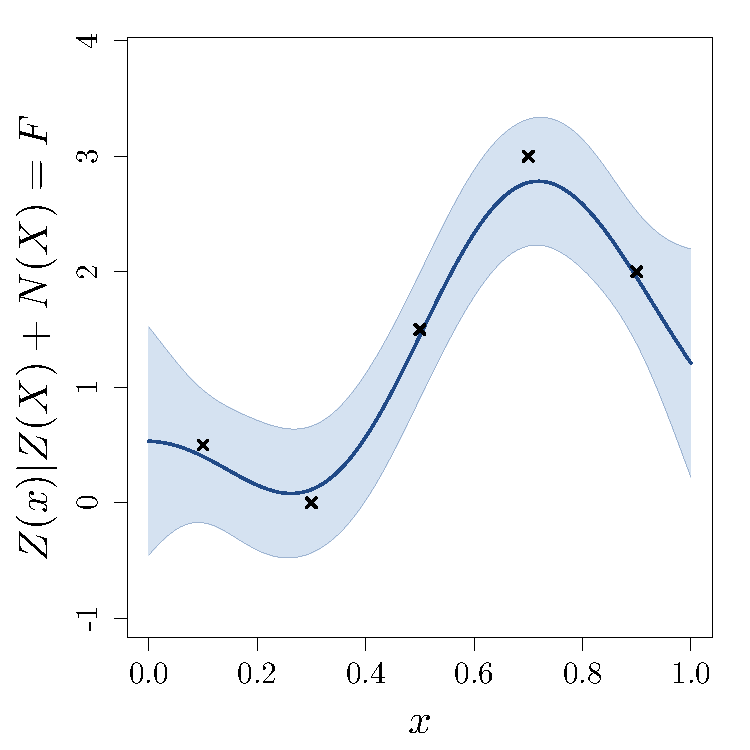
\includegraphics[width=\textwidth]{figures/ch2_GPRnoise01}
                \caption{$\tau^2 = 0.1$}
        \end{subfigure}%
        \caption{Influence of the signal to noise ratio in Gaussian process regularisation models. The covariance of $Z$ is squared exponential ($\sigma^2=1$, $\theta=0.2$) and $N(X)$ are independent centred Gaussian random variables with variance $\tau^2$. The observation points are not represented on the left panel in order to distinguish the small but non zero confidence intervals at prediction points.}
        \label{fig:GPRnoise}
\end{figure}

\paragraph{}
One consequence of adding observation noise is to improve the conditioning of matrix that has to be inverted. For example, if we consider a Gaussian process regression model without observation noise that has two observations very close one to each other, the two columns of the covariance matrix associated to these observations will tend to be equal and the matrix will not be invertible numerically. On the other hand, adding some observation noise greatly improves the conditioning since it implies adding a value $\tau^2$ on the diagonal (typically around $1e-5$) of the covariance matrix and the columns are not similar any more. 


%%%%%%%%%%%%%%%%%%%%%%%%%%%%%%%%%%%%%%%%%%%%%%%%%%%%%%%%%%%%
\section{Practical issues}
\paragraph{}
Making predictions from a Gaussian process regression model as in Eq.~\ref{eq:GPR} or \ref{eq:noisyGPR} requires to compute the $n \times n$ matrix $k(X,X)$ and to invert it. As a consequence, the space complexity is $O(n^2)$ and the time one is $O(n^3)$. As a consequence, the computational limitations for using such models only depends on the number of observation points. In practice, the storage limitation happens to be more restrictive than the computational one and the maximum number of observations that can be handled is somewhere between 1000 to 10000 depending on the computational resources.

\paragraph{}
Another practical issue that often arises is bad conditioning of the covariance matrix which makes the computation of the inverse troublesome. We have seen that, by definition, a covariance matrix is positive semi-definite: for all $\alpha$, we have $\alpha^t k(X,X) \alpha \geq 0$. If the limit case $\alpha^t k(X,X) \alpha = 0$ is reached for a $\alpha \neq 0$, then $\alpha$ corresponds to an eigenvector with null eigenvalue and the matrix is not invertible. This is for example the case if one observation point is repeated twice (say $X_i = X_j$): the $i^{\mathrm{th}}$ and $j^{\mathrm{th}}$ columns of the covariance matrices are thus equal and we have $\alpha^t k(X,X) \alpha = 0$ for $\alpha_i=1$, $\alpha_j=-1$ and $\alpha_k=0$ for $k \neq i$ and $k \neq j$. The probabilistic interpretation is that $\alpha^t Z(X)$ is a random variable with zero variance (since it is null) and thus the multivariate distribution of $Z(X)$ is degenerated. 

\paragraph{}
Bad conditioning of $k(X,X)$ can be interpreted as an information given twice to the model. In practice, two points that are close to each other may lead to numerical instability even if they are not at the exact same location. As a rule of thumb, the more regular the sample paths are, the more sensitive the model will be to close-by observations. A procedure that is helpful when this kind of trouble arise is then: 
\begin{enumerate}
	\item Compute the eigenvectors $P_i$ associated to null eigenvalues: the points associated to non-zero coefficients indicate the redundant ones.
	\item Check if the observations satisfy the equation given by the eigenvectors $P_i^t F = 0$
	\begin{itemize}
		\item if they do, some of them can be removed without any loss of information until the matrix becomes invertible.
		\item if they don't, then the choice of the kernel is not appropriate to the data. Some observation noise may be added to the model to account for the between the assumption and the observations.
	\end{itemize}
\end{enumerate}
Note that it is helpful to conceive distance between input space points $x$ and $y$ not as the usual Euclidean distance but as pseudo-distance given by the correlation\footnote{For more details, see \emph{Mahalanobis distance}.} between the process values $Z(x)$ and $Z(y)$. For instance, when using a periodic kernel, two points that are exactly one period apart have a correlation of 1: they correspond to the exact same information and from a correlation point of view they can be considered to be at the same location. As a consequence, considering a kernel where the correlation drops faster (for example reducing the values of the length scale parameters or changing from a Gaussian kernel to a Mat\'ern one) will improve the conditioning of the covariance matrix and can be sufficient to make it invertible.


%%%%%%%%%%%%%%%%%%%%%%%%%%%%%%%%%%%%%%%%%%%%%%%%%%%%%%%%%%%%
\section{Multi-outputs Gaussian processes}
\paragraph{}
All this chapter is based on the fact that the random vector $(Y(x),Y(X))$ is multivariate normal. As a consequence, all previous results can be extended to the case of multi-output Gaussian processes. For example, let us assume that you observe over time the temperature in two cities $A$ and $B$ that are located in the same country. If we assume that some Gaussian processes $T_A(t)$ and $T_B(t)$ are good priors for these temperatures, we can of course build two separate models but we would loose the correlation between them. An alternative approach is to assume that the couple $(T_A,T_B)$ is Gaussian and to make one unique joint model: the prediction for the city $A$ is thus given by the conditional distribution $T_A(t)|T_A(X_A), T_B(X_B)$. In order to fully describe the distribution of the Gaussian vector $(T_A(t),\ T_A(X_A),\ T_B(X_B))$, one need to specify the cross-covariance between the $T_A$ and $T_B$: $k_{AB}(t,t') = \Cov[T_A(t),T_B(t')]$. Note that the latter is not symmetric ($k_{AB}(t,t') \neq k_{AB}(t',t)$) but satisfies $k_{AB}(t,t') = k_{BA}(t',t)$. The previous GPR formulas still apply and write:
\begin{equation}
	\begin{split}
		m_A(t) &= \E[T_A(t)|T_A(X_A) \shorteq F_A, T_B(X_B) \shorteq F_B] \\
		&= \begin{pmatrix}
			k_A(t,X_A) & k_{AB}(t,X_B)
		\end{pmatrix}
		\begin{pmatrix}
			k_A(X_A,X_A) & k_{AB}(X_A,X_B) \\
			k_{AB}(X_A,X_B)^t & k_{B}(X_B,X_B) \\
		\end{pmatrix}^{-1}
		\begin{pmatrix}
			F_A \\
			F_B \\
		\end{pmatrix}\\
		c_A(t,t') &=  \Cov[T_A(t),T_A(t')|T_A(X_A) \shorteq F_A, T_B(X_B) \shorteq F_B] \\
		&= k_A(t,t') - 
		\begin{pmatrix}
			k_A(t,X_A) & k_{AB}(t,X_B)
		\end{pmatrix} \\
		&  \hspace{4cm} \times
		\begin{pmatrix}
			k_A(X_A,X_A) & k_{AB}(X_A,X_B) \\
			k_{AB}(X_A,X_B)^t & k_{B}(X_B,X_B) \\
		\end{pmatrix}^{-1}
		\begin{pmatrix}
			k_A(t',X_A)^t \\
			k_{AB}(t',X_B)^t
		\end{pmatrix}
	\end{split}
	%\label{eq:multiGPR}
\end{equation}

An other point of view that stresses the similarity with the usual Gaussian process regression models is to augment the input space: in this case, one could consider that one observation of the temperature is associated to one time point $t$ and one label $l \in \{ A, B\}$: the prior is then given by a process $T(t,l)$ with a kernel $k((t,l),(t',l'))$. With such settings, the usual formula are unchanged. One illustration is shown in the left panel of Figure~\ref{fig:multiGPR}.

\begin{figure}
        \centering
        \begin{subfigure}[b]{0.44\textwidth}
                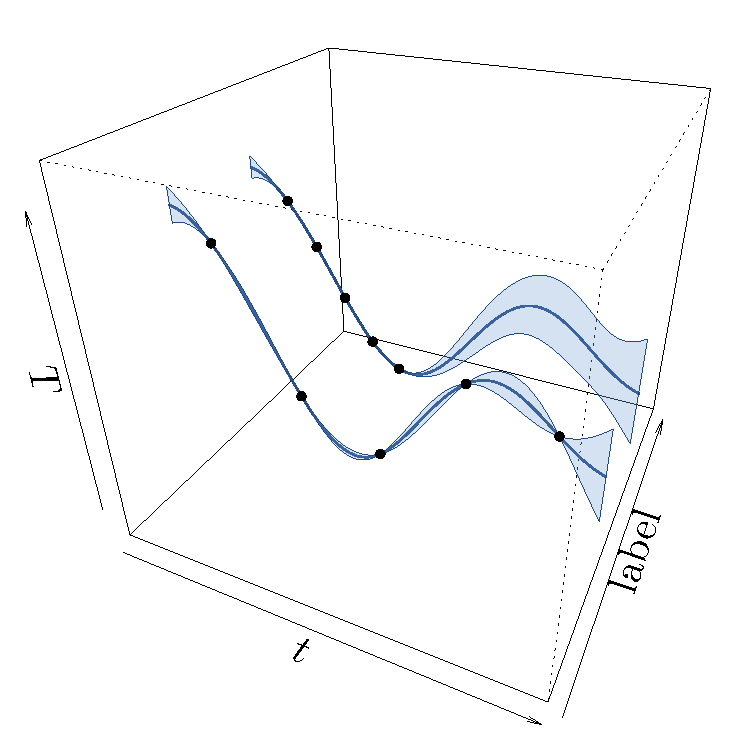
\includegraphics[width=\textwidth]{figures/ch2_multiGPR}
                \caption{Example of multi-output GPR. \\ \ }
        \end{subfigure}%
        \hspace{1cm}       
        \begin{subfigure}[b]{0.44\textwidth}
                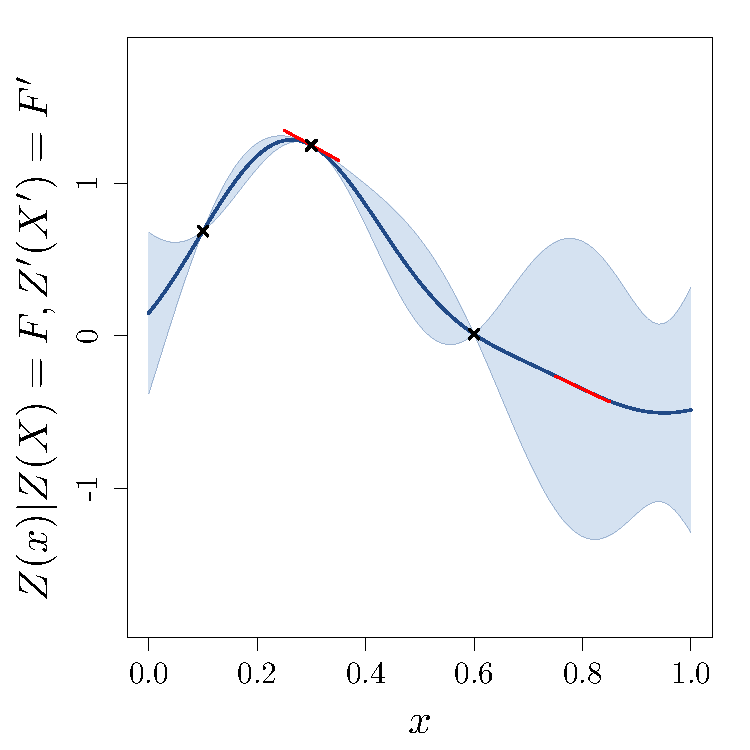
\includegraphics[width=\textwidth]{figures/ch2_derGPR}
                \caption{Example of GPR with two observations of the derivative in $X'=(0.3\ 0.8)$.}
        \end{subfigure}
        \caption{Multi-output Gaussian process regression.}
        \label{fig:multiGPR}
\end{figure}

\paragraph{}
In practice, this can be useful in various situations. A common one is given by the use of numerical simulators with different levels of accuracy for approximating one phenomenon. In this situation, even if the high fidelity simulator is more accurate, it can be interesting to take into account in the model observations of the low-fidelity one since they often are much less expensive to compute. Another situation is when one observe both the value of the process and its derivative. In this case, it is interesting to consider the couple $(Z,Z')$ and to compute the predictions based on the conditional distribution $Z(x)|Z(X),Z'(X')$. This is illustrated on the right panel of Figure~\ref{fig:multiGPR}.

%%%%%%%%%%%%%%%%%%%%%%%%%%%%%%%%%%%%%%%%%%%%%%%%%%%%%%%%%%%%
%%%%%%%%%%%%%%%%%%%%%%%%%%%%%%%%%%%%%%%%%%%%%%%%%%%%%%%%%%%%
\chapter{Model parameters estimation}
\paragraph{}
In the previous chapters, we have seen how to build a Gaussian process regression model using a given kernel. Since these kernels depend on parameters, it is legitimate to wonder what parameter values should be chosen. For the sake of clarity, we focus in this section on the estimation of a kernel with parameters $(\sigma^2,\theta)$, but the methods detailed here are of course valid for other types of kernels.

%%%%%%%%%%%%%%%%%%%%%%%%%%%%%%%%%%%%%%%%%%%%%%%%%%%%%%%%%%%%
\section{Cross Validation} 
\paragraph{}
A natural approach for choosing a kernel and its parameter is to compare the prediction error (or the normality of the residuals) of various models and then to choose the one with the lowest error. In practice, there is often no test set dedicated to learning the parameters and cross validation methods can be applied. A typical example of cross validation is \emph{leave-one-out} where we consider the sub-models $m_i$ based on all training points except the $i^{th}$ one. Error is then defined as:
\begin{equation}
MSE_{LOO} = \frac{1}{n} \sum_{i=1}^n (m_i(x_i) - Y_i)^2.
\end{equation}
As we have seen previously, the variance parameter has no influence on the mean predictor so minimizing the $MSE_{LOO}$ is only useful for estimating the length scale parameter. Since for a given $x$ the standardized residuals of a GPR model $(m(x)-f(x))/\sqrt(v(x))$ should be $\mathcal{N}(0,1)$, it is possible to start from a model with arbitrary covariance (say 1) and then to reset it such that the empirical leave-one-out standardized residuals have a variance exactly equal to 1. This can be achieve by setting
\begin{equation}
 \sigma^2_{CV} = \frac{1}{n} \sum_{i=1}^n \frac{(m_i(x_i) - Y_i)^2}{v_i(x_i)}.
\end{equation}

\begin{example}
	Given the design of experiments $X=(0.1,\  0.3,\  0.5,\  0.7,\  0.9)^t$ and the observations $Y = (0.69,\ 1.25,\  0.5,\ -0.25,\ 0.31)^t$, the leave-one-out estimation of a Mat\'ern 5/2 kernel gives $\sigma^2_{CV}=0.55 $ and $\theta_{CV}=0.28$. The resulting model is illustrated on the left panel of Figure \ref{fig:paramEstim}.
\end{example}

\paragraph{}
It has been shown in the literature\footnote{F. Bachoc, \emph{Cross Validation and Maximum Likelihood estimations of hyper-parameters of Gaussian processes with model misspecification.} Computational Statistics \& Data Analysis 66 (2013): 55-69.} that cross validation can perform better than maximum likelihood (see bellow) when the kernel is misspecified.

%%%%%%%%%%%%%%%%%%%%%%%%%%%%%%%%%%%%%%%%%%%%%%%%%%%%%%%%%%%%
\section{Maximum likelihood estimation} 
\paragraph{}
The principle of likelihood is to quantify the adequacy between a distribution and some observations. Let $f_Y$ be a probability density function depending on some parameters $p$ (such as a mean, a variance, a rate, ...) and  $y_1,\dots,y_n$ be independent observations from a random variable. The likelihood is defined as: 
\begin{equation}
 	L(p) = \prod_{i=1}^n f_Y(y_i;p).
\end{equation} 
A high value of $L(p)$ indicates that the observations are likely to be drawn from $f_Y(.;p)$, whereas a value of 0 means that the observations ``cannot'' come from it.  

\paragraph{}
In Gaussian process regression, it is quite common to observe only one sample of the random vector $Z(X)=F$. The distribution of this vector is often considered as centred so it depends only on its kernel. Since the kernels typically depends on a variance $\sigma^2$ and a length scale $\theta$, the likelihood writes:
\begin{equation}
 	L(\sigma^2, \theta) = f_{Z(X)}(F ; \sigma^2, \theta) = \frac{1}{\displaystyle | 2 \pi k(X,X)|^{1/2}} \exp \left(-\frac12 F^t k(X,X)^{-1} F  \right).
\end{equation} 
where $k(.,.)$ depends on $\sigma^2$ and $\theta$. As can be seen from this expression, the likelihood is equal to the probability density function but seen as a function of the distribution's parameters. The likelihood can take extremely small values and it is often helpful to consider log-likelihood to avoid numerical issues:
\begin{equation}
 	\log (L (\sigma^2, \theta)) = - \frac{n}{2} 2 \pi - \frac{1}{2}  \log(|k(X,X)|) -\frac12 F^t k(X,X)^{-1} F .
\end{equation} 
This expression can be further simplified without changing the optimization solution $(\sigma^2, \theta)$: maximizing the (log-)likelihood is equivalent to minimizing
\begin{equation}
 	\ell (\sigma^2, \theta) =  \log(|k(X,X)|) + F^t k(X,X)^{-1} F
\end{equation} 
which we will call the reduced likelihood.

\paragraph{}
Since $\sigma^2$ is a factor in the kernel expression $k(x,y)=\sigma^2 r(x,y)$, the reduced likelihood writes
\begin{equation}
 	\ell (\sigma^2, \theta) =  \log(\sigma^{2n} |r(X,X)|) + \sigma^{-2} F^t r(X,X)^{-1} F.
\end{equation} 
For a given value of $\theta$ the optimal value of $\sigma$ can be obtained analytically by getting the value for which the derivative is null:
\begin{equation}
 	 \frac{\partial \ell}{\partial \sigma^2} (\sigma^2_{MLE}, \theta) = 0 \Leftrightarrow \sigma^2_{MLE} = \frac1n F^t r(X,X)^{-1} F.
\end{equation} 
Unfortunately, other kernel parameters such as $\theta$ cannot be estimated in a similar fashion and, as for cross-validation, a numerical procedure is required to optimize them.

\begin{example}
	For the same settings as in the previous figures, maximum likelihood estimation gives $\sigma^2_{MLE}=0.24 $ and $\theta_{MLE}=0.15)$. As shown on Figure \ref{fig:paramEstim}, this lead to a model that is quite different from the obtained with cross validation where $\sigma^2_{CV}=0.55 $ and $\theta_{CV}=0.28)$.
	\begin{figure}[ht!]
        \centering
        \begin{subfigure}[b]{0.44\textwidth}
                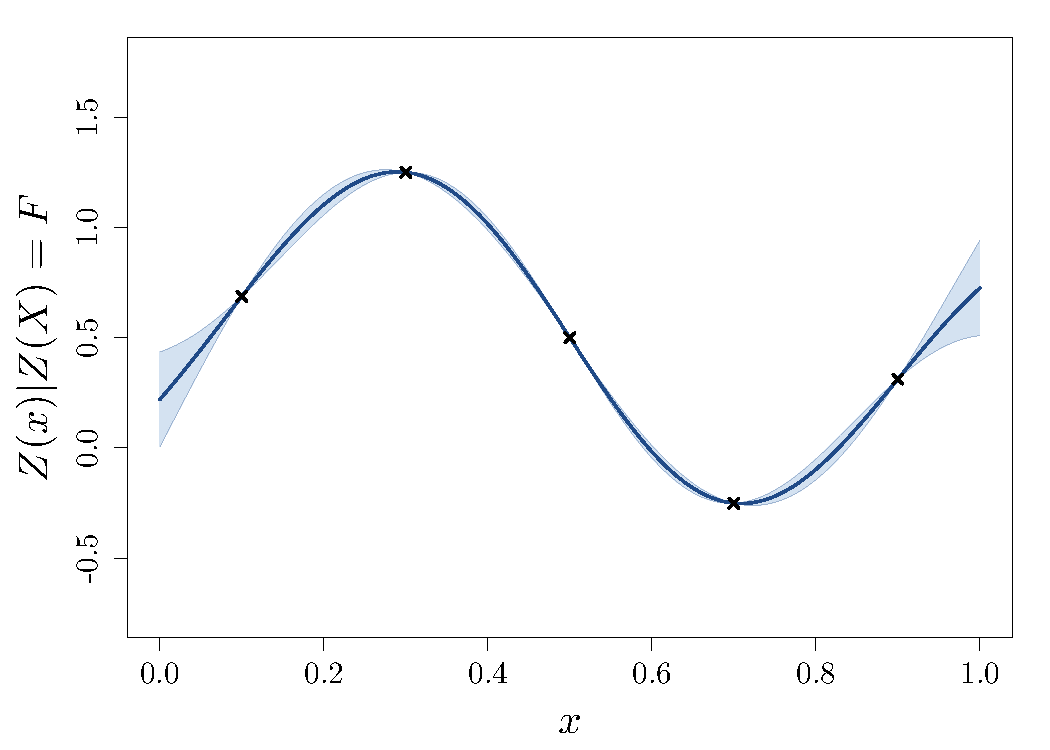
\includegraphics[width=\textwidth]{figures/ch3_CV}
                \caption{Model obtained with cross validation. \\ \ }
        \end{subfigure}%
        \hspace{1cm}       
        \begin{subfigure}[b]{0.44\textwidth}
                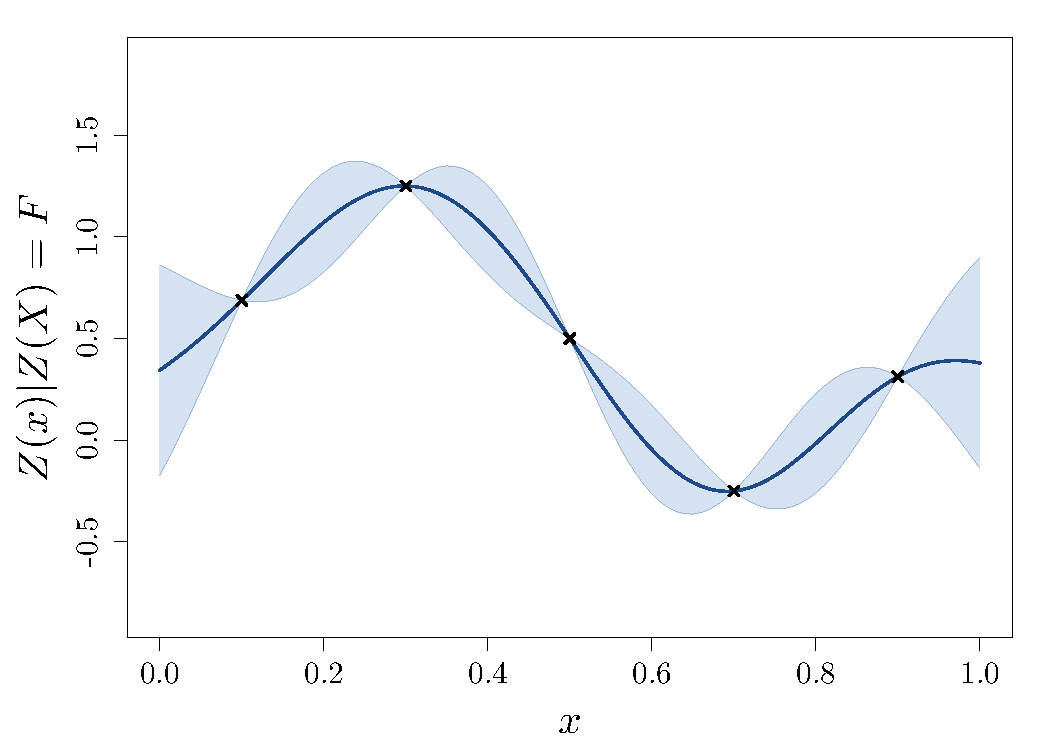
\includegraphics[width=\textwidth]{figures/ch3_MLE}
                \caption{Model obtained with maximum likelihood estimation.}
        \end{subfigure}
        \caption{Example of parameter estimation of a Mat\' ern 5/2 kernel.}
        \label{fig:paramEstim}
	\end{figure}
\end{example}


% %%%%%%%%%%%%%%%%%%%%%%%%%%%%%%%%%%%%%%%%%%%%%%%%%%%%%%%%%%%%
% \section{the variogram framework} 
% \paragraph{}
% \todo{everything}


%%%%%%%%%%%%%%%%%%%%%%%%%%%%%%%%%%%%%%%%%%%%%%%%%%%%%%%%%%%%
%%%%%%%%%%%%%%%%%%%%%%%%%%%%%%%%%%%%%%%%%%%%%%%%%%%%%%%%%%%%
\chapter{Model validation}
\paragraph{}
One question of utmost importance in modelling is the validation of the model. It means that we have to make sure that the predictions made by the model actually make sense and that we can rely on the model for further analysis or for decision taking. The principle of validation is to compare the prediction of the model and the actual value of the function on a set of points that has not been used for building the model.  

\paragraph{}
One asset of the Gaussian process regression model is to provide not only a mean value but a prediction variance as well. It means that the two of them should be analysed when it comes to model validation. We will now discuss two options, with or without a dedicated test set. 

%%%%%%%%%%%%%%%%%%%%%%%%%%%%%%%%%%%%%%%%%%%%%%%%%%%%%%%%%%%%
\section{With test set}
When a test set $X_t$ is available, the $Q_2$ criterion is often used for validating the mean predictor:
\begin{equation}
Q_2 = 1 - \frac{\sum (F_t - m(X_t))^2}{\sum (F_t - \mathrm{mean}(F_t))^2}.
\end{equation}
The value of this criterion is equal to one when the model predictions are perfectly accurate ($m(X_t) = F_t$) and equal to zero when a constant value ($\mathrm{mean}(F_t)$) can predict as well as the model. Negative values may arise when using this criterion, they imply that a constant function can predict better than the model.

\paragraph{}
Validating the conditional covariance can be done by analysing if the observations predictions follow the distribution predicted by the model. According to the model, $F_t$ is normally distributed with mean $m(X_t)$ and covariance matrix $c(X_t,X_t)$ so the standardised residuals $c(X_t,X_t)^{-1/2}(F_t-m(X_t))$ should be independent standard Gaussian. This can be tested by applying classical statistical tests or graphical representations such as QQ-plots.

%%%%%%%%%%%%%%%%%%%%%%%%%%%%%%%%%%%%%%%%%%%%%%%%%%%%%%%%%%%%
\section{Without test set}
A dedicated test set is not always available, especially if the function is costly to evaluate. One option is then to consider leave-one-out methods or, more generally, a cross validation approach. The principle of leave-one-out is to build a model with all the points of the design of experiments except one and then to compare the model prediction at that point with the actual observation value. This procedure is then be repeated for every point of the design. As previously, the $Q_2$ criterion can be used to measure the model error and the residuals can be standardised before applying normality tests. However, the model does not provide a joint distribution for the errors and they have to be standardised separately.

\paragraph{}
In the same spirit, it is possible to apply cross validation methods with subsets of $k$ points of the design. This allows to test if the joint distribution predicted by the model actually makes sense.

\paragraph{}
One flaw of cross validation methods is that, if the design is conceived to fill the space, the error is computed at a point that is the  less favourable for the model. For example, if we consider a set of 11 points $X=(0,0.1,...,1)$ equally spaced in $D = [0,1]$, the further one point of $D$ can be from $X$ is $0.05$ but leave-one-out will compute errors for points that are twice further from the observations. 


%%%%%%%%%%%%%%%%%%%%%%%%%%%%%%%%%%%%%%%%%%%%%%%%%%%%%%%%%%%%
%%%%%%%%%%%%%%%%%%%%%%%%%%%%%%%%%%%%%%%%%%%%%%%%%%%%%%%%%%%%
\chapter{Kernel design}

As stated in Theorem~\ref{thm:loeve}, any symmetric positive semi-definite function can be seen a the covariance a Gaussian process and thus can be used in a Gaussian process regression model. However, a direct proof of the positive definiteness of a function is often intractable. We will discuss in this chapter four options for designing new kernels.

%%%%%%%%%%%%%%%%%%%%%%%%%%%%%%%%%%%%%%%%%%%%%%%%%%%%%%%%%%%%
\section{Finite dimensional kernels}
Mercer theorem is an important result on kernels: it states that a continuous kernel can always be written as an infinite sum 
\begin{equation}
	k(x,y) = \sum_{i=1}^\infty \lambda_i \phi_i(x) \phi_j(x)
\end{equation}
where the $\lambda_i$ are positive scalars and where the $\phi_i$ are continuous square integrable functions.

\paragraph{}
If a kernel can be written as a finite sum, then the kernel is said to be \emph{finite dimensional}. For such kernels, the sample paths will live in a finite dimensional space. Among the kernels presented in Table \ref{tab:ker1d} and \ref{tab:kerdimd}, the constant kernel $k_{cst}(x,y)=\sigma^2$ and the linear one $k_{lin}(x,y)=\sigma^2 xy$ are the only of finite dimensional kernels. Their samples are respectively constant functions and straight lines going through the origin. 

\paragraph{}
In practice, it is very easy to generate finite dimensional kernels. Let $\varepsilon$ be a random variable with distribution $\mathcal{N}(0,1)$ and $g$ be any given function $D \rightarrow \mathds{R}$, then $Z(x)=\varepsilon g(x)$ is a Gaussian process with kernel $k(x,y)=g(x)g(y)$. This can be generalised as follow:
\begin{property}[finite dimensional kernels]
    Let $g(.) = (g_1(.),\dots,g_d(.))^t$ be a $d$-dimensional vector of functions $D \rightarrow \mathds{R}$ and let $D$ be a $d \times d$ symmetric positive semi-definite matrix. Then
    \begin{equation}
        k(x,y) = g(x)^t C g(y)
    \end{equation}
    is a valid covariance function over $D \times D$. In particular, if $C$ is a diagonal matrix with coefficients $\sigma_i^2$, then $k$ writes
        \begin{equation}
        k(x,y) = \sum_{i=1}^d \sigma_i^2 g_i(x)g_i(y).
    \end{equation}
\end{property}
\begin{proof}
    Let $\varepsilon$ be a $d$-dimensional centred Gaussian vector with covariance matrix $C$, then $Z(x)= g(x)^t \varepsilon$ is a Gaussian process and its kernel is $g(x)^t C g(y)$.
\end{proof}

\paragraph{}
Using finite dimensional kernels for GPR implies that a limited number of observations is sufficient to know the process perfectly everywhere. This is illustrated in the following example:
\begin{example}
    According to the previous property, $k(x,y) = \sum_{i=1}^2 \cos(i \pi x )\cos(i \pi y ) + \sin(i \pi x ) \sin(i \pi y )$ is a valid covariance function. Some samples an models based on such kernels are represented in the following graphs:
        \begin{figure}[ht!]
        \centering
        \begin{subfigure}[t]{0.30\textwidth}
                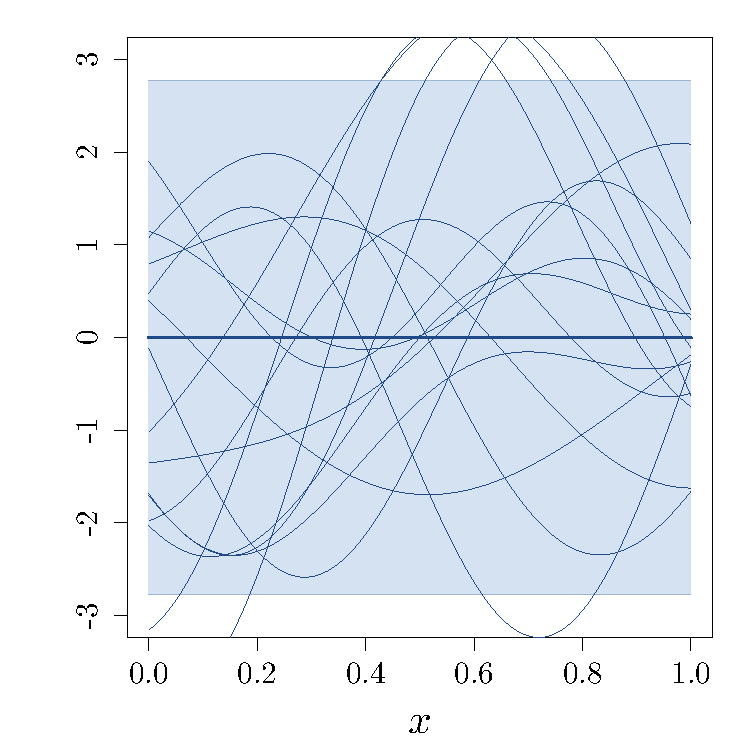
\includegraphics[width=\textwidth]{figures/ch5_finitedim0}
                \caption{Prior distribution.}
        \end{subfigure}%
        \hspace{0.2cm}       
        \begin{subfigure}[t]{0.30\textwidth}
                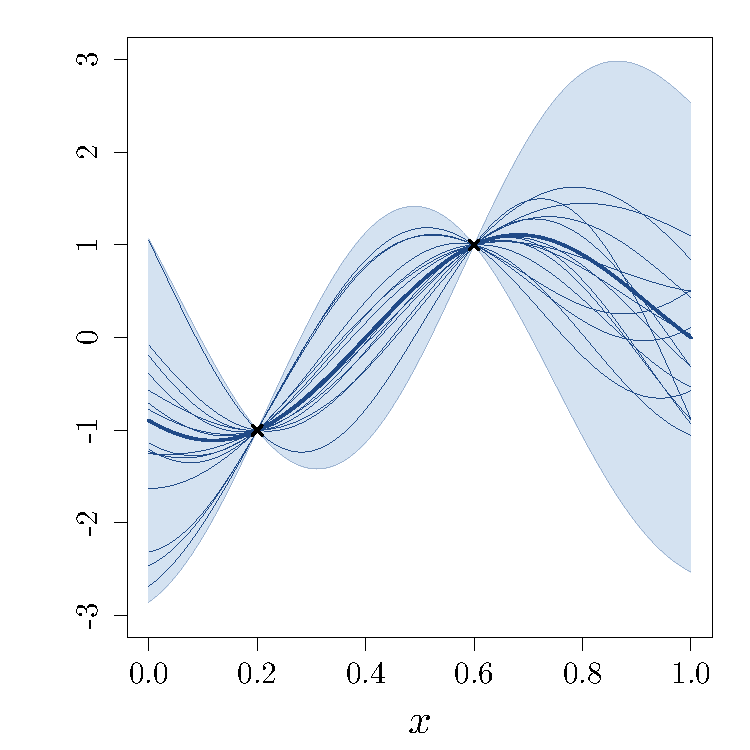
\includegraphics[width=\textwidth]{figures/ch5_finitedim2}
                \caption{GPR with 2 observations.}
        \end{subfigure}%
        \hspace{0.2cm}       
        \begin{subfigure}[t]{0.30\textwidth}
                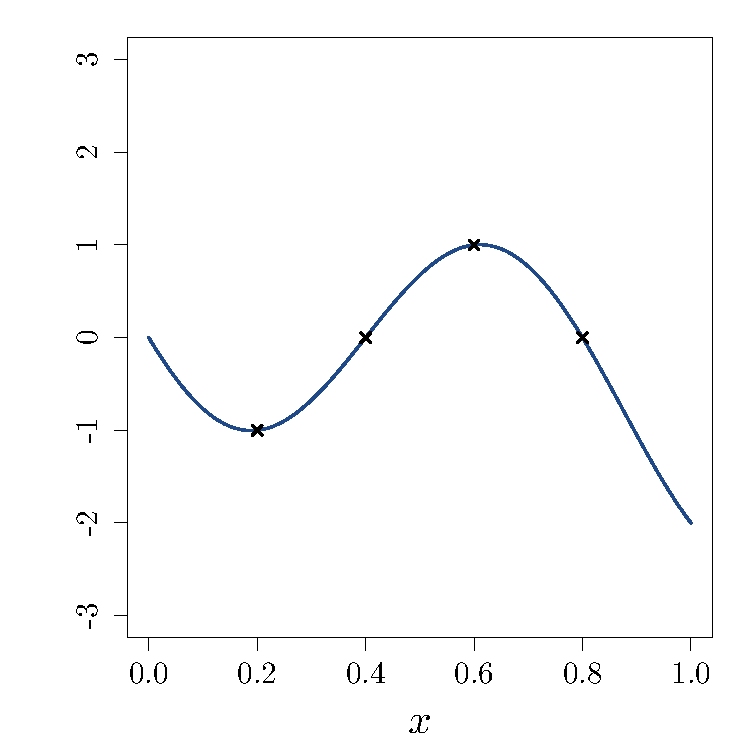
\includegraphics[width=\textwidth]{figures/ch5_finitedim4}
                \caption{GPR with 4 observations.}
        \end{subfigure}
        \caption{Prior and conditional distributions of a finite dimensional kernel. The design of experiments is $X=(0.2, 0.4, 0.6, 0.8)^t$ and the observations are $Y=(-1,0,1,0)^t$.}
        \label{fig:ch5_findimkern}
    \end{figure}
\end{example}

%%%%%%%%%%%%%%%%%%%%%%%%%%%%%%%%%%%%%%%%%%%%%%%%%%%%%%%%%%%%
\section{Bochner theorem}
Bochner theorem gives a mapping between positive measures and stationary positive semi-definite functions. We recall that stationary kernels are kernels that can be written as a function of the variable $x-y$. Since it shall not be a source of confusion, we will use the notation $k(t) = k(t,0)$ and thus $k(x,y)$ may be written $k(x-y)$.
\begin{theorem}
\label{thm:bochner}
The Fourier transform of a positive measure $\mu$ is a stationary symmetric positive semi-definite function. Reciprocally, the inverse Fourier transform of a stationary symmetric positive semi-definite function is a positive measure.
\end{theorem}
In practice, we are interested in real valued processes so will always consider symmetric measures $\mu$. This theorem is very useful to prove that many usual kernels are positive semi-definite. For example:
\begin{itemize}
        \item The squared exponential kernel is the Fourier transform of a Gaussian bell.
        \item Kernels from the Mat\'ern family with parameter $\nu$ are the Fourier transform of 
\begin{equation}
S(\omega) =  \left( \frac{2 \nu}{\ell ^2} + \omega ^2 \right)^{-(\nu+1/2)}.
\label{eq:SDmat}
\end{equation}
        \item The constant kernel $k(t) = \sigma^2$ is the Fourier transform of the dirac measure $\delta_{x,y}$.
        \item The white noise kernel is the Fourier transform of a constant measure.
\end{itemize}

Bochner theorem is not the only result linking positive definite function and other specific class of functions. One can cite for example the link between kernels and completely monotone functions but such developments are out of the scope of this document. 


%%%%%%%%%%%%%%%%%%%%%%%%%%%%%%%%%%%%%%%%%%%%%%%%%%%%%%%%%%%%
\section{Making new from old}
Although it can be difficult to prove that a function is positive semi-definite there are many transformations preserving this property that can be applied to well known off-the-shelf kernels, such as the ones described in Section~\ref{sec:kernels}, in order to create new ones.

%%%%%%%%%%%%%%%%%%%%%%%%%%%%%%%%%%%%%%%%%%%%%%%%%%%%%%%%%%%%
\subsection{Sum of kernels}

\begin{property}[sum of kernels]
	Let $k_1$ and $k_2$ be two kernels defined on $D \times D$. Then 
	\begin{equation}
		k(x,y) = k_1(x,y) + k_2(x,y)
	\end{equation}
	is a valid covariance function on $D \times D$.
\end{property}
The proof of this proposition is straightforward: let $Z_1$ and $Z_2$ be independent random processes with kernels $k_1$ and $k_2$, then $k$ is the kernel of $Z(x) = Z_1(x) + Z_2(x)$.

\paragraph{}
The practical interest of summing kernels is highlighted in the following example:

\begin{example}
	The $CO_2$ concentration in the air has been monitored monthly since 1958 at the Mauna Loa observatory in Hawaii. The resulting  660 observation are shown on the left panel of Figure \ref{fig:CO2}. If we want to forecast the $CO_2$ concentration in the next few years, one can try to fit a GPR model with a squared exponential kernel to these data points. However, finding an appropriate length scale for this model will be cumbersome: one can either notice the long term raising trend and decide to choose a large value for the length scale parameter. However, such model will be unable to cope with the high frequency oscillations and the prediction intervals of the model will be very wrong (cf Figure \ref{fig:CO2}). On the other hand, one can choose a small length scale to reflect this high frequency phenomenon but the model then totally misses the trend. 

	\begin{figure}[ht!]
        \centering
        \begin{subfigure}[t]{0.30\textwidth}
                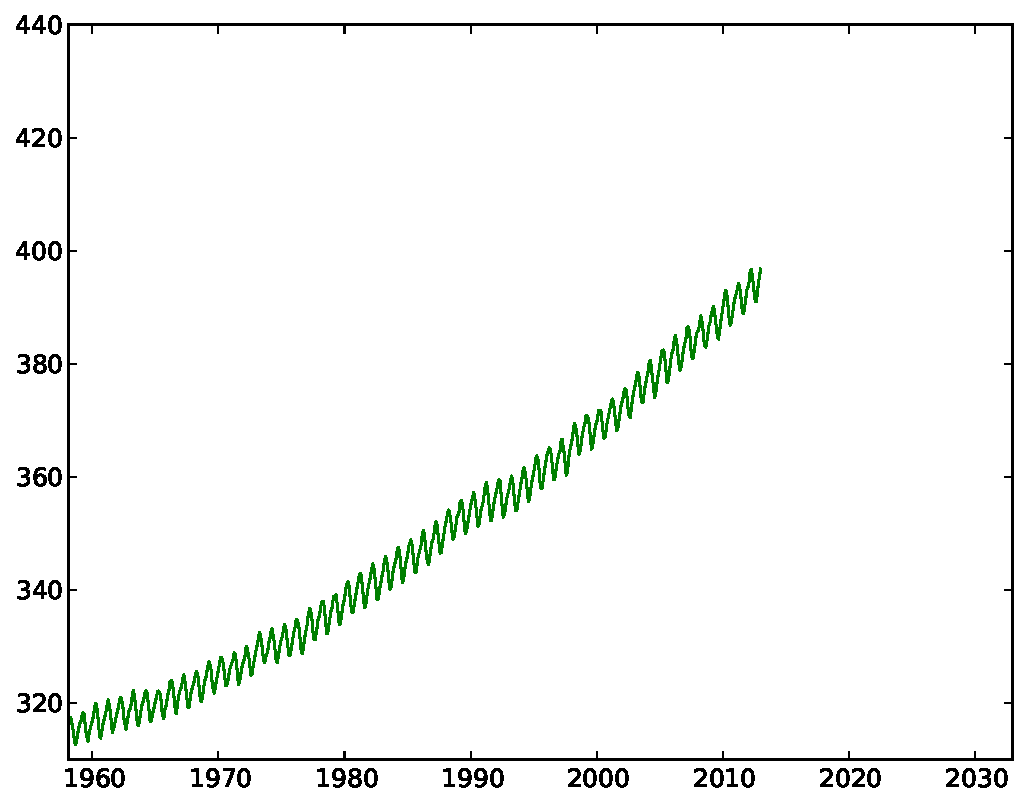
\includegraphics[width=\textwidth]{figures/python/CO2-data}
                \caption{Dataset.}
        \end{subfigure}%
        \hspace{0.2cm}       
        \begin{subfigure}[t]{0.30\textwidth}
                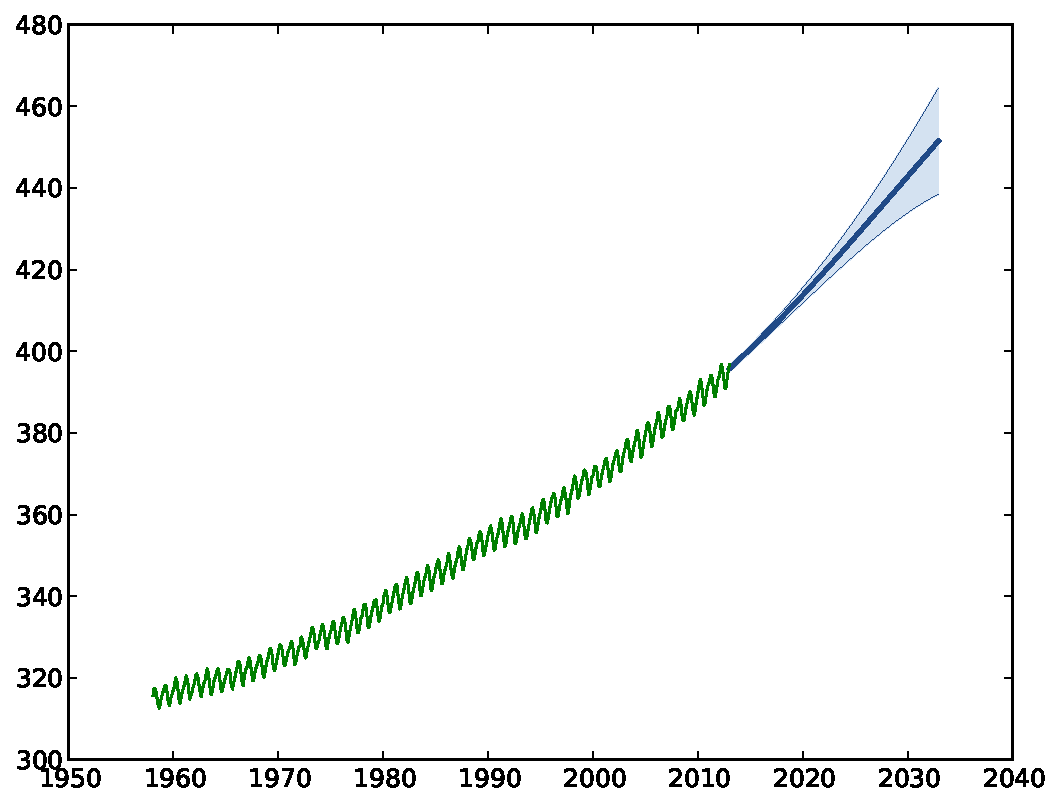
\includegraphics[width=\textwidth]{figures/python/CO2-rbfb}
                \caption{Model with large length scale.}
        \end{subfigure}
        \hspace{0.2cm}       
        \begin{subfigure}[t]{0.30\textwidth}
                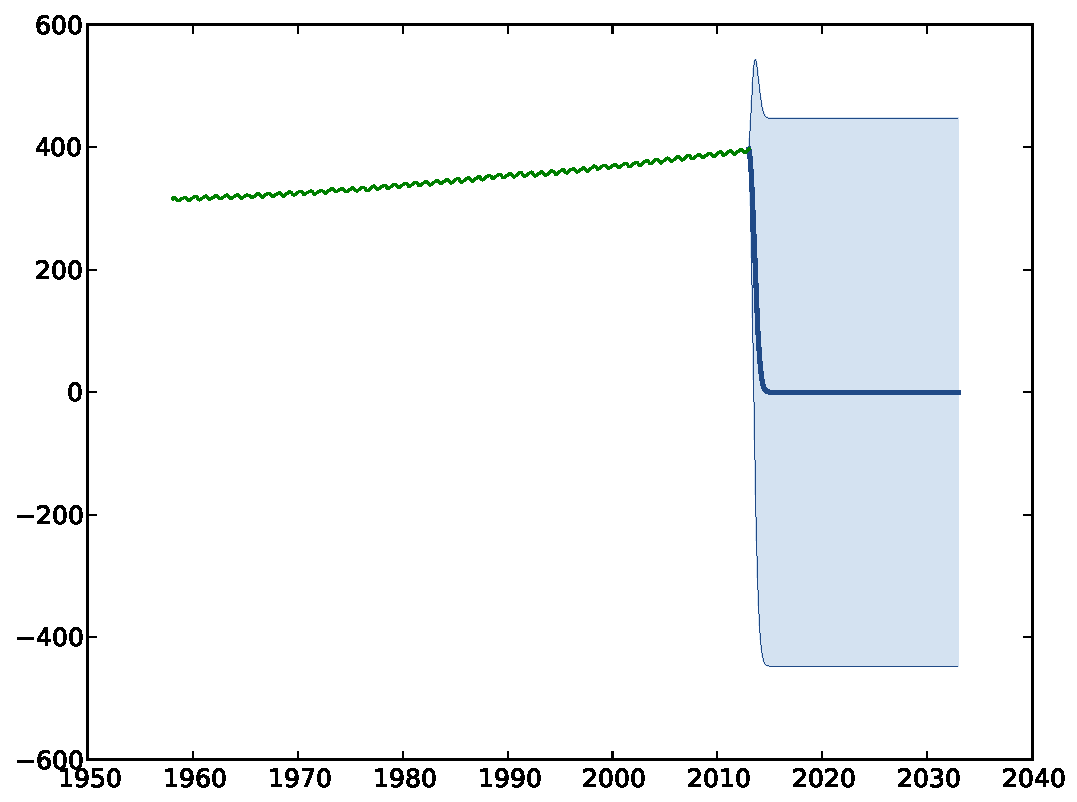
\includegraphics[width=\textwidth]{figures/python/CO2-rbfa}
                \caption{Model with small length scale.}
        \end{subfigure}
        \caption{Original data set and models based on a single squared exponential kernel.}
        \label{fig:CO2}
	\end{figure}

	\paragraph{}
	Alternatively, one can consider the sum of two kernels with small and large length scale and to account for the two frequencies that can be found in the signal. This leads to a much better model as can be seen on Figure \ref{fig:CO2top}. This model can be further improved by adding a periodic kernel to account for the one year periodicity ($CO_2$ concentration is always higher during summer).

	\begin{figure}[ht!]
        \centering
        \begin{subfigure}[t]{0.44\textwidth}
                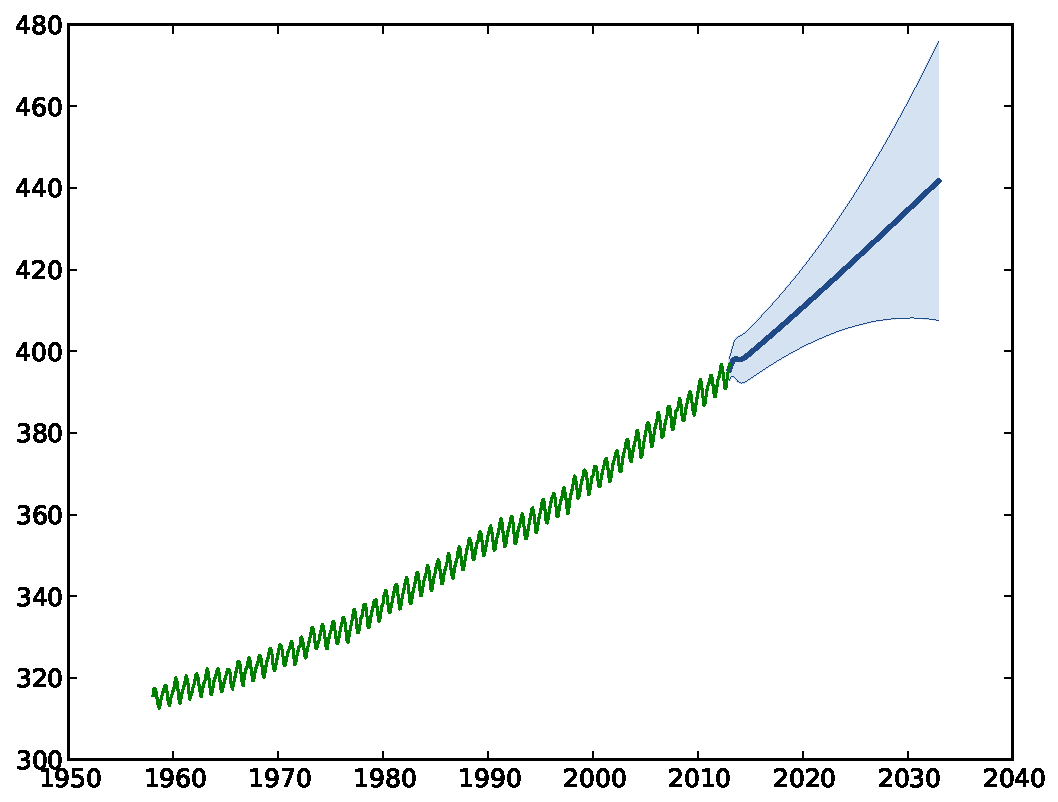
\includegraphics[width=\textwidth]{figures/python/CO2-rbfab}
                \caption{Sum of kernels with different length scales. }
        \end{subfigure}%
        \hspace{1cm}       
        \begin{subfigure}[t]{0.44\textwidth}
                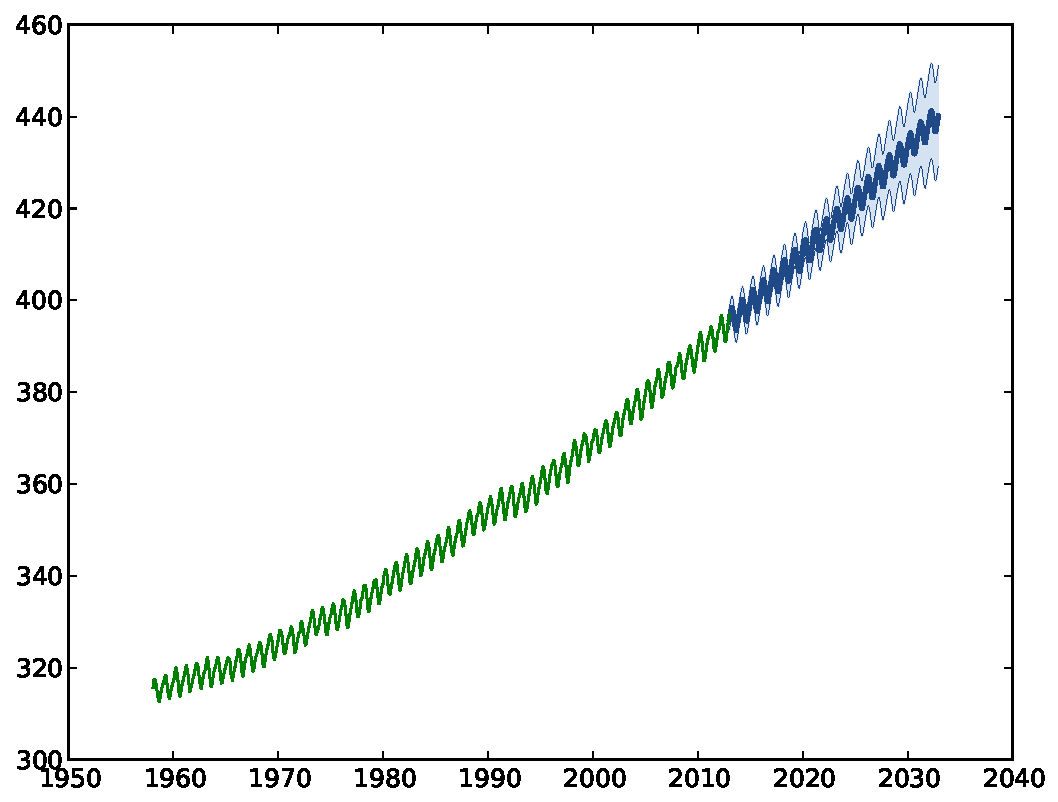
\includegraphics[width=\textwidth]{figures/python/CO2-rbfabpq}
                \caption{sum of three kernels including a periodic one.}
        \end{subfigure}
        \caption{Models based on sums of kernels.}
        \label{fig:CO2top}
	\end{figure}
\end{example}

Another way of summing kernels is to consider kernels defined on different spaces and to sum them to obtain a kernel over the tensor space:
\begin{property}[tensor sum of kernels]
	Let $k_1$ and $k_2$ be two kernels defined respectively on $D_1 \times D_1$ and $D_2 \times D_2$. Then 
	\begin{equation}
		k((x_1,x_2),(y_1,y_2)) = k_1(x_1,y_1) + k_2(x_2,y_2)
	\end{equation}
	is a valid covariance function on $(D_1 \times D_2) \times (D_1 \times D_2)$.
\end{property}

\paragraph{}
Such kernels can be useful in various situations. Of course, if we know that the function to approximate is additive (ie if it writes $f(x)= \sum f_i(x_i)$), then choosing an additive kernel is an easy way to account for this information. This is for illustrated in Example \ref{ex:kernSum}. 

\paragraph{}
Another situation where tensor additive kernels can be of great help is for approximating functions with high dimensional input parameters. When using regular kernels, such as squared exponential or a Mat\'ern, each observation only influences its neighbourhood. As a consequence, the number of points required to approximate a function with a given precision grows exponentially with the input dimension. On the other hand, a model based on an additive kernel (for example a sum of one dimensional squared exponential or Mat\'ern) will only require the number of training point to grow linearly with the dimension. The drawback is that an additive model is less flexible and can at best fit the additive component of a function that is not fully additive.

\begin{example}
	We consider the test function $f(x) = \sin(4 \pi x_1) + \cos(4 \pi x_2) + 2 x_2$ over $[0,1]^2$ and a set of 12 observation points (see figure below). To account for the periodicity of the test function, we use a tensor additive kernel based on two squared exponential kernels: $k(x,y) = \sigma^2_1 \exp \left(- \frac{(x_1-y_1)^2}{2 \theta_1^2} \right) + \sigma^2_2 \exp \left(- \frac{(x_2-y_2)^2}{2 \theta_2^2} \right)$. Maximum likelihood estimation gives the following parameter values : $(\sigma^2_1,\ \theta_1^2,\ \sigma^2_2 ,\ \theta_2) = (0.88,\ 0.11,\ 0.92,\ 0.11)$. The resulting mean and prediction variance are given in the following figure. As shown on the right panel graph, the prediction variance can be zero even at some prediction points where there is no observation (e.g. the point $x=(0.08,0.66)$). This is because the knowledge of the value of an additive function at 3 vertices of a rectangle $(x_1,x_2)$, $(x_1,y_2)$ and $(y_1,y_2)$ is sufficient to know the value on the fourth vertex: $f(y_1,x_2)=f(x_1,x_2)+f(y_1,y_2)-f(x_1,y_2)$.
	\begin{figure}[ht!]
        \centering
        \begin{subfigure}[t]{0.29\textwidth}
                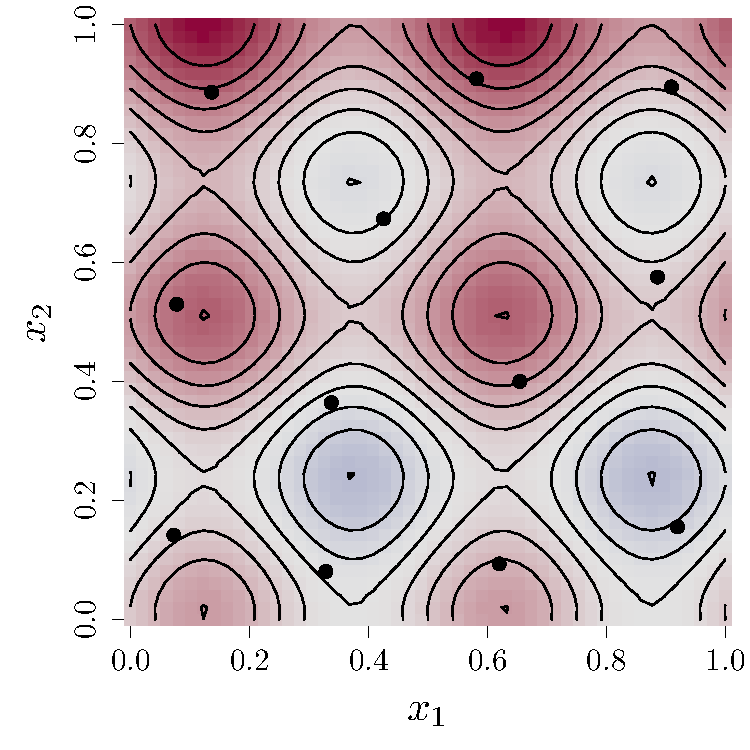
\includegraphics[height=4.2cm]{figures/ch5_addfunc}
                \caption{Test function. \\ \ }
        \end{subfigure}%
        \hspace{0.2cm}       
        \begin{subfigure}[t]{0.29\textwidth}
                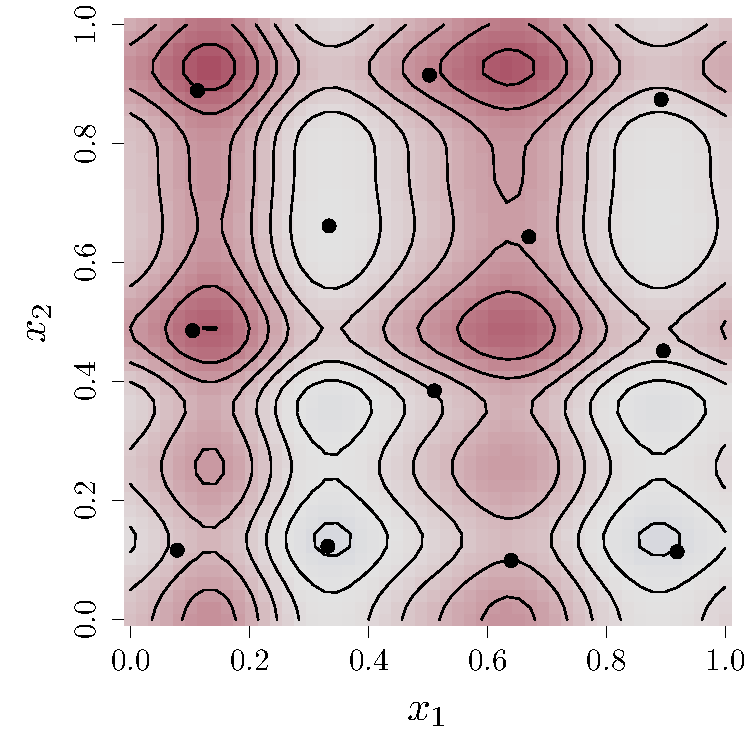
\includegraphics[height=4.2cm]{figures/ch5_addmean}
                \caption{Mean predictor. \\ \ }
        \end{subfigure}
        \hspace{0.2cm}       
        \begin{subfigure}[t]{0.29\textwidth}
                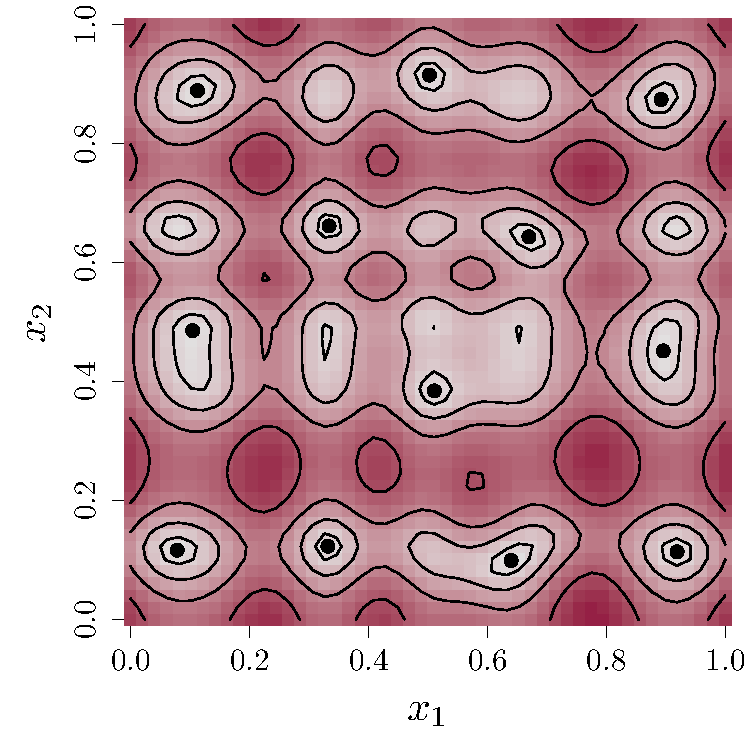
\includegraphics[height=4.2cm]{figures/ch5_addsd}
                \caption{Predicted Standard deviation (times 4).}
        \end{subfigure}
        \hspace{0.2cm}   
        \begin{subfigure}[t]{0.05\textwidth}
                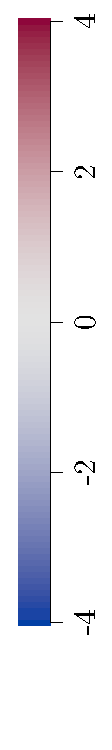
\includegraphics[height=4.2cm]{figures/ch5_addlegend}
        \end{subfigure}
        
        \caption{Test function and associated model. The color scale is the same for all graphs.}
        \label{fig:ch5additive}
	\end{figure}
    \label{ex:kernSum}
\end{example}
One striking property of kernels that are sums of kernels is that the model can be split in sub-models corresponding to conditional Gaussian distributions. This can be illustrated on a follow-up of the previous example: since the kernel writes $k(x,y) = k_1(x_1,y_1) + k_2(x_2,y_2)$, the best predictor writes:
\begin{equation}
\begin{split}
m(x) &= \big(k_1(x_1,X_1) + k_2(x_2,X_2) \big) \big( k_1(X_1,X_1) + k_2(X_2,X_2) \big)^{-1} F\\
&= k_1(x_1,X_1) \big( k_1(X_1,X_1) + k_2(X_2,X_2) \big)^{-1} F + k_2(x_2,X_2) \big( k_1(X_1,X_1) + k_2(X_2,X_2) \big)^{-1} F\\
&= \E [Z_1(x_1) | Z_1(X_1) + Z_2(X_2)  \shorteq  F] + \E [Z_2(x_2) | Z_1(X_1) + Z_2(X_2)  \shorteq  F] \\
&= m_1(x_1) + m_2(x_2)
\end{split}
\end{equation}
where $Z_1$ and $Z_2$ are two independent centred Gaussian processes with kernels $k_1$ and $k_2$. For the sub-model $m_1$, the influence of $Z_2$ can be seen as observation noise. Furthermore, it is possible to associate prediction variance to each sub-models:
\begin{equation}
\begin{split}
v_i(x_i) &= \Var [Z_i(x_i) | Z_1(X_1) + Z_2(X_2)  \shorteq  F] \\
&= k_i(x_i,x_i) -  k_i(x_i,X_i) \big( k_1(X_1,X_1) + k_2(X_2,X_2) \big)^{-1} k_i(X_i,x_i)
\end{split}
\end{equation}  
This can be of particular interest when the input space is more that 2 dimensional since it allows a graphical representation of the influence of each variable, as in Figure~\ref{fig:ch5adddec}.
    \begin{figure}[ht!]
        \centering
        \begin{subfigure}[t]{0.45\textwidth}
                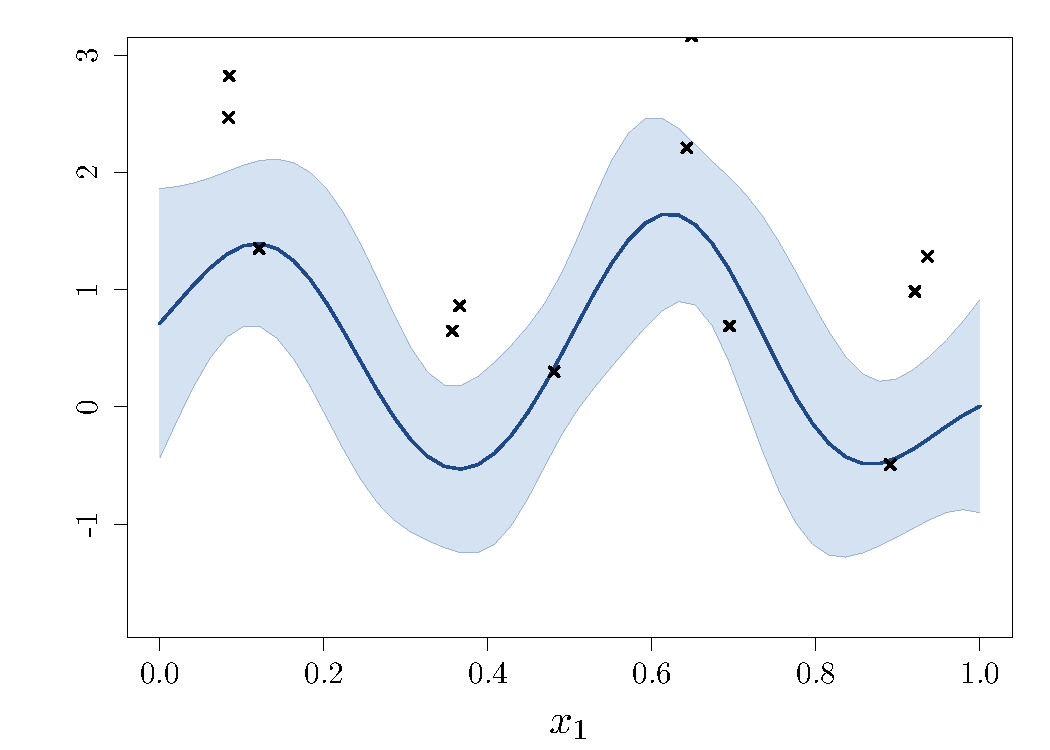
\includegraphics[width=\textwidth]{figures/ch5_addSubModel1}
                \caption{Sub-model 1: $Z_1(x_1)|Z(X) \shorteq F$. }
        \end{subfigure}%
        \hspace{1cm}       
        \begin{subfigure}[t]{0.45\textwidth}
                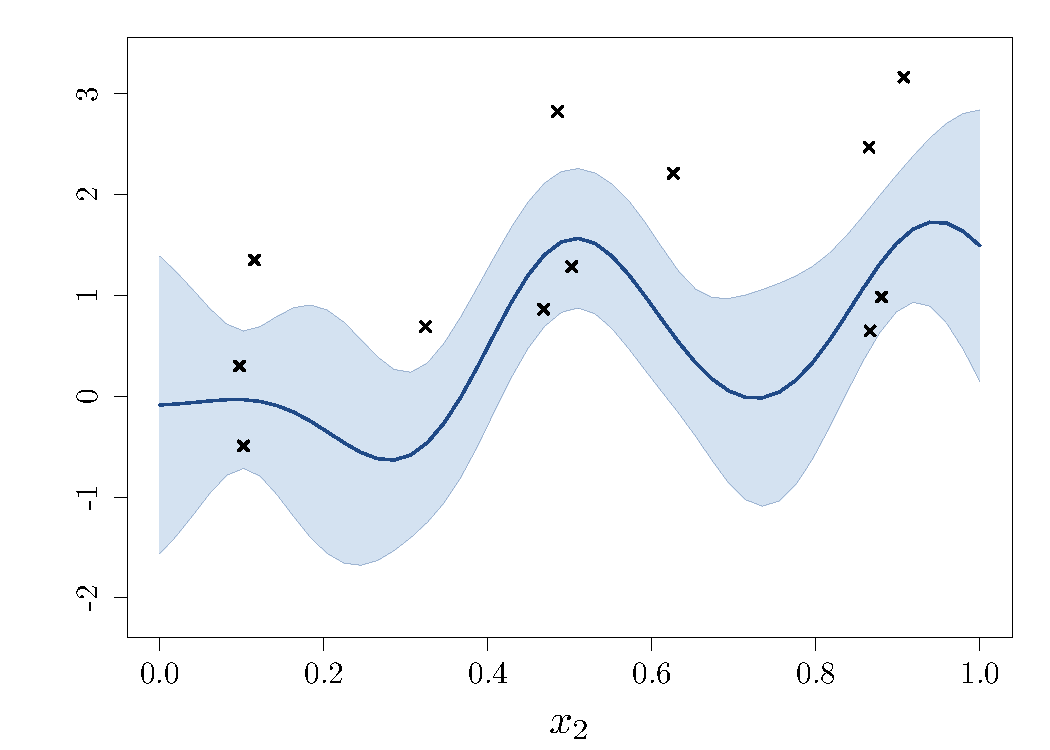
\includegraphics[width=\textwidth]{figures/ch5_addSubModel2}
                \caption{Sub-model 2: $Z_2(x_2)|Z(X) \shorteq F$.}
        \end{subfigure}
        \caption{Decomposition of the GPR model of Example \ref{ex:kernSum} as a sum of sub-models.}
        \label{fig:ch5adddec}
    \end{figure}

%%%%%%%%%%%%%%%%%%%%%%%%%%%%%%%%%%%%%%%%%%%%%%%%%%%%%%%%%%%%
\subsection{Product of kernels}
As for the sum of kernels, the product of kernel can be conceived either for kernels defined on the same space or for kernels defined on different spaces.
\begin{property}[product of kernels]
	Let $k_1$ and $k_2$ be two kernels defined on $D \times D$. Then 
	\begin{equation}
		k(x,y) = k_1(x,y) \times k_2(x,y)
	\end{equation}
	is a valid covariance function on $D \times D$.
\end{property}
\begin{example}
	The Mat\'ern 5/2 kernel and the cosine function are both positive definite. As a consequence, their product 
	\begin{equation}
	k_{prod}(x,y) = \sigma^2 \cos \left( \frac{x-y}{\theta_1} \right) \left(1 + \frac{\sqrt{5}|x-y|}{\theta_2} + \frac{5|x-y|^2}{3 \theta_2^2} \right) \exp \left(- \frac{\sqrt{5}|x-y|}{\theta_2} \right)
	\end{equation}
	is also positive semi-definite. The following figure shows this kernel as well as some sample paths. It can be noticed that they oscillate without being periodic.
	\begin{figure}[ht!]
        \centering
        \begin{subfigure}[t]{0.45\textwidth}
                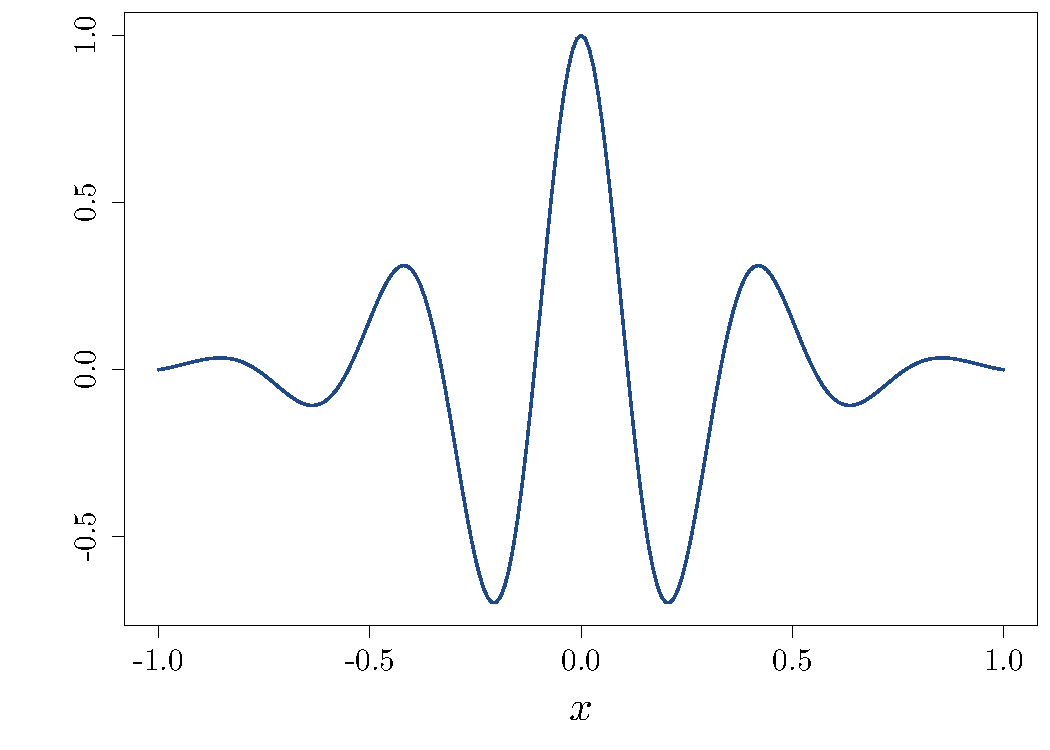
\includegraphics[width=\textwidth]{figures/ch5_prodKern}
                \caption{Kernel $k_{prod}(x,0)$. \\ \ }
        \end{subfigure}%
        \hspace{1cm}       
        \begin{subfigure}[t]{0.45\textwidth}
                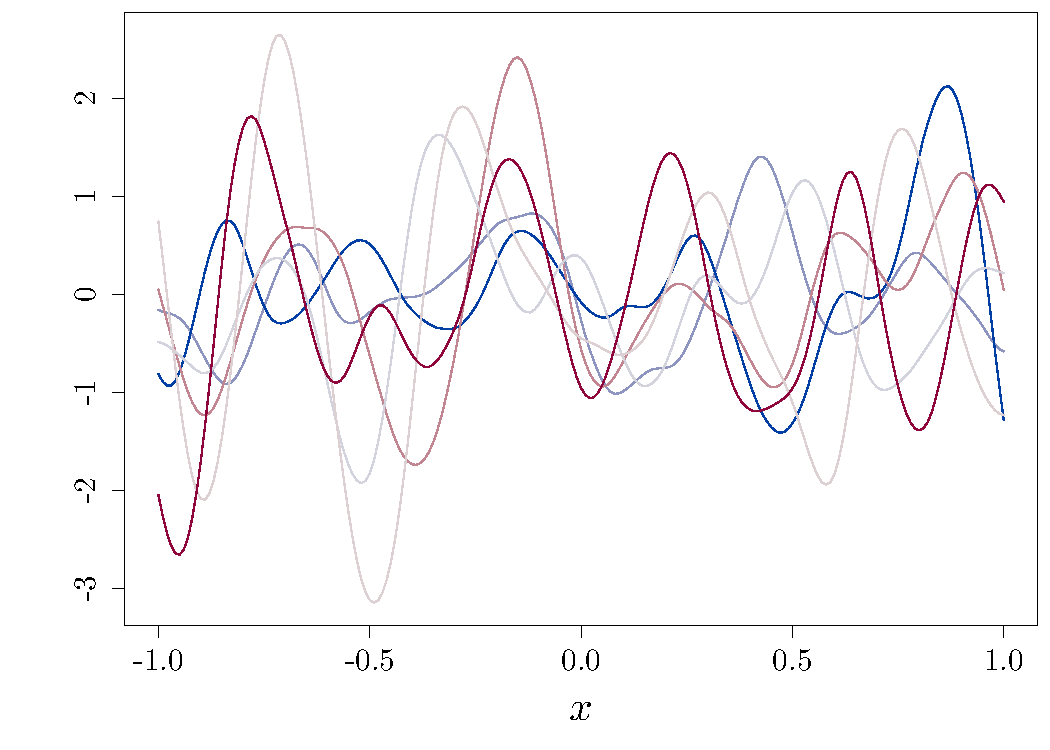
\includegraphics[width=\textwidth]{figures/ch5_prodSimu}
                \caption{Random samples. \\ \ }
        \end{subfigure}
        \caption{Example of product kernel. The parameters are $\sigma^2=1$, $\theta_1=0.07$ and $\theta_1=0.3$.}
        \label{fig:ch5product}
	\end{figure}
\end{example}

\begin{property}[tensor product of kernels]
	Let $k_1$ and $k_2$ be two kernels defined respectively on $D_1 \times D_1$ and $D_2 \times D_2$. Then 
	\begin{equation}
		k((x_1,x_2),(y_1,y_2)) = k_1(x_1,y_1) \times k_2(x_2,y_2)
	\end{equation}
	is a valid covariance function on $(D_1 \times D_2) \times (D_1 \times D_2)$.
\end{property}
This property can be used to create higher dimensional kernels from low dimensional ones. For example, one can multiply two squared exponential kernels to create a two dimensional one: 
\begin{equation}
\begin{split}
k(x,y) &= \sigma^2_1 \exp \left(- \frac{(x_1-y_1)^2}{2 \theta_1^2} \right) \times \sigma^2_2 \exp \left(- \frac{(x_2-y_2)^2}{2 \theta_2^2} \right)\\
& = \sigma^2_1 \sigma^2_2 \exp \left(-\frac12 \left( \frac{(x_1-y_1)^2}{\theta_1^2} + \frac{(x_2-y_2)^2}{\theta_2^2} \right) \right)
\end{split}
\end{equation}
 The attentive reader will have recognize here the expression of the anisotropic 2 dimensional squared exponential kernel. 

%%%%%%%%%%%%%%%%%%%%%%%%%%%%%%%%%%%%%%%%%%%%%%%%%%%%%%%%%%%%
\subsection{Kernel rescaling}
We have seen that kernels often have an input rescaling parameter $\theta$ called the length scale. In practice, this rescaling does not have to be linear and one can introduce a function to account for this input change:
\begin{property}[kernel warping]
    Let $k_1$ be a kernel defined on $D_1 \times D_1$ and $g$ be a function $D \rightarrow D_1$. Then 
    \begin{equation}
        k(x,y) = k_1(g(x),g(y))
    \end{equation}
    is a valid covariance function on $D \times D$.
\end{property}
As previously the proof is extremely simple: if $Z_1$ is a process with kernel $k_1$, then $k_1(g(x),g(y))$ is the kernel of $Z(g(x))$.

\paragraph{}
This kind of transformation is useful if one wants to introduce non stationarity in models, as illustrated in the left panel of Figure \ref{fig:ch5rescaling}.

\paragraph{}
Similarly, kernel typically include a variance parameter that correspond to an output rescaling. As for the length scale, this rescaling is not necessarily a constant:
\begin{property}[kernel output rescaling]
    Let $k_1$ be a kernel defined on $D \times D$ and $g$ be a function $D \rightarrow \mathds{R}$. Then 
    \begin{equation}
        k(x,y) = g(x)g(y)k_1(x,y)
    \end{equation}
    is a valid covariance function on $D \times D$.
\end{property}
Two simple proofs can be given for this property: one based on Gaussian processes where $g(x)g(y)k_1(x,y)$ is seen as the covariance of a process $g(x)Z(x)$, and another one where it is seen as the product of the finite dimensional kernel $g(x)g(y)$ with the kernel $k_1(x,y)$. This type of transformation is illustrated in Figure \ref{fig:ch5rescaling}.

\begin{figure}[ht!]
    \centering
    \begin{subfigure}[t]{0.45\textwidth}
            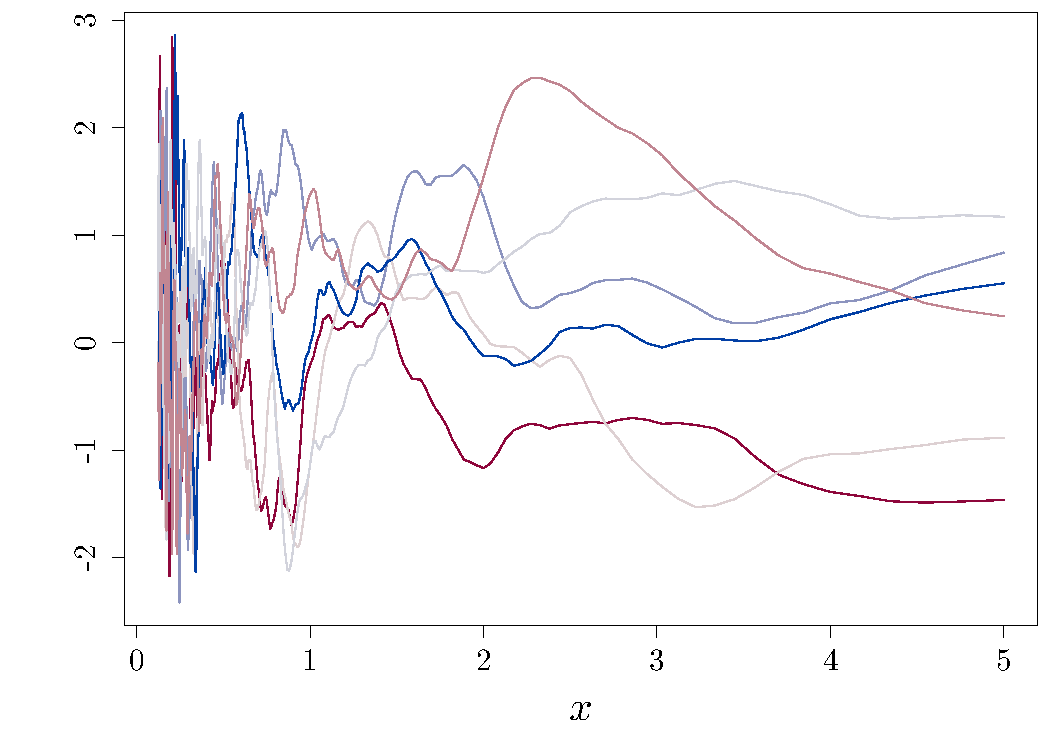
\includegraphics[width=\textwidth]{figures/ch5_rescKern1}
            \caption{Input rescaling: $k(x,y) = k_1(1/x,1/y)$ }
    \end{subfigure}%
    \hspace{1cm}       
    \begin{subfigure}[t]{0.45\textwidth}
            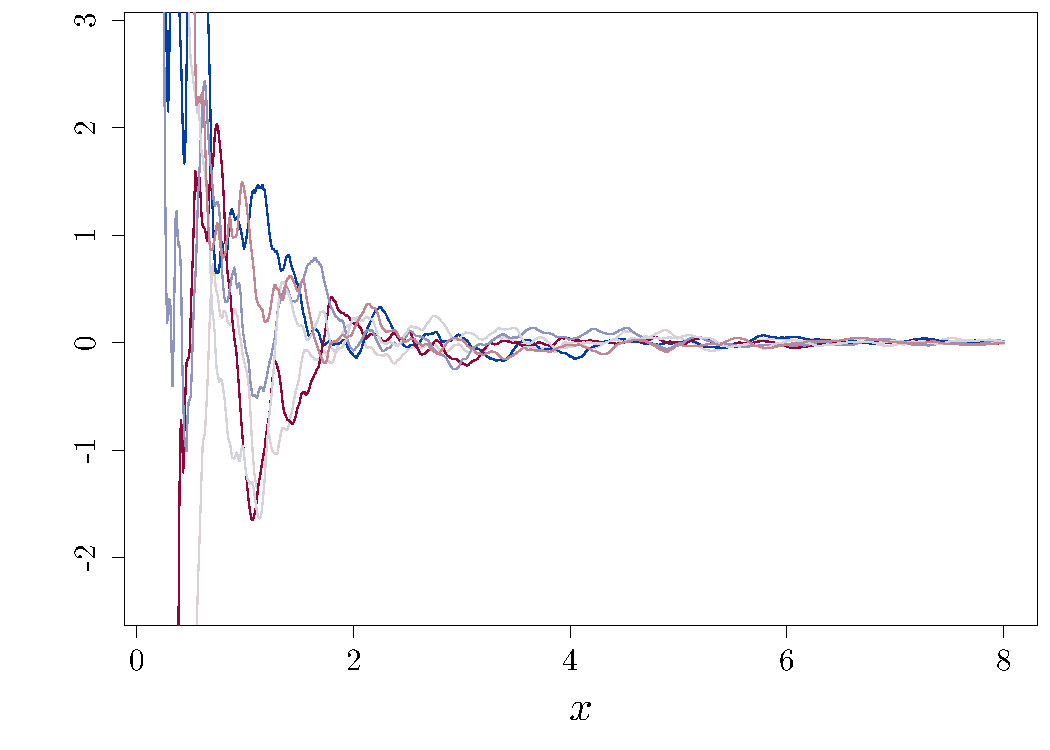
\includegraphics[width=\textwidth]{figures/ch5_rescKern2}
            \caption{output rescaling. $k(x,y) = 1/(xy) k_1(x,y)$  }
    \end{subfigure}
    \caption{Examples of processes based on kernels with input/output rescaling. The initial kernel  $k_1$ is a Mat\'ern 3/2 with parameters $\sigma^2=1$ and $\theta=0.2$. In both case, the function use for rescaling is $g:\ x \rightarrow 1/x$.}
    \label{fig:ch5rescaling}
\end{figure}


%%%%%%%%%%%%%%%%%%%%%%%%%%%%%%%%%%%%%%%%%%%%%%%%%%%%%%%%%%%%
\section{Linear transformation of Gaussian processes}
We will discuss in this section other transformations that can be applied to kernel to encapsulate more sophisticated information.


\begin{property}[transformation operator]
    Let $L$ be a linear operator that is well defined on samples of $Z$. Then\footnote{to be rigorous, we also need some continuity conditions on $L$. However, the required material is out of the scope of this course.} 
    \begin{equation}
        k(x,y) = L_x(L_y(k(x,y)))
    \end{equation}
    is a valid covariance function. In this equation, $L_x$ denote the operator $L$ applied to $x \mapsto k(x,y)$.
    \label{prop:lintransform}
\end{property}
This property can be useful in various situations: if the function to approximate has some particular properties and if it is possible to build an operator that transform any function in a function satisfying these properties, then, under the hypothesis of Property \ref{prop:lintransform}, it is possible to design an appropriate kernel. We will now illustrate this on two examples:
\begin{example}[symmetric model]
    This example comes from the R package \emph{kergp}. Let $L$ be a transformation that associate to any function over $\mathds{R}^2$ a function symmetric with respect to both axis:
    \begin{equation}
       L(g)(x_1,x_2) = g(|x_1|,|x_2|).
    \end{equation}
    Now, let $k$ be a Gaussian kernel over $\mathds{R}^2 \times \mathds{R}^2$. According to the previous property, 
    \begin{equation}
       k_{sym}(x,y) = L_x(L_y(k(x,y))) = \sigma^2 \exp \left( {-\frac{(|x_1|-|y_1|)^2}{2 \theta_1^2 }} \right) \exp \left({-\frac{(|x_2|-|y_2|)^2}{2 \theta_2^2 }} \right)
    \end{equation}
    is a valid covariance function. This is illustrated in Figure \ref{fig:ch5sym}.
    \begin{figure}[ht!]
        \centering
        \begin{subfigure}[t]{0.30\textwidth}
                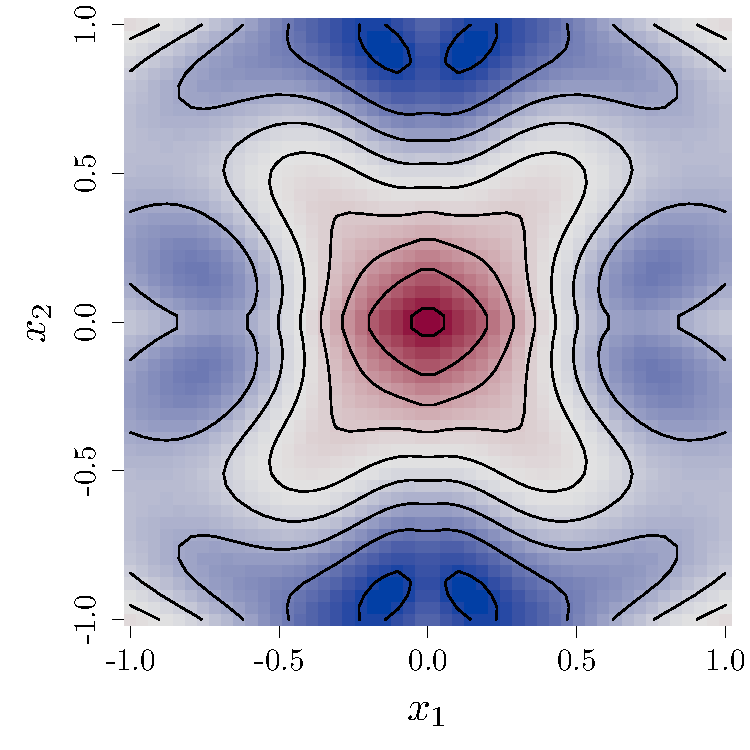
\includegraphics[width=\textwidth]{figures/ch5_symSample}
                \caption{Example of sample path.}
        \end{subfigure}%
        \hspace{0.2cm}       
        \begin{subfigure}[t]{0.30\textwidth}
                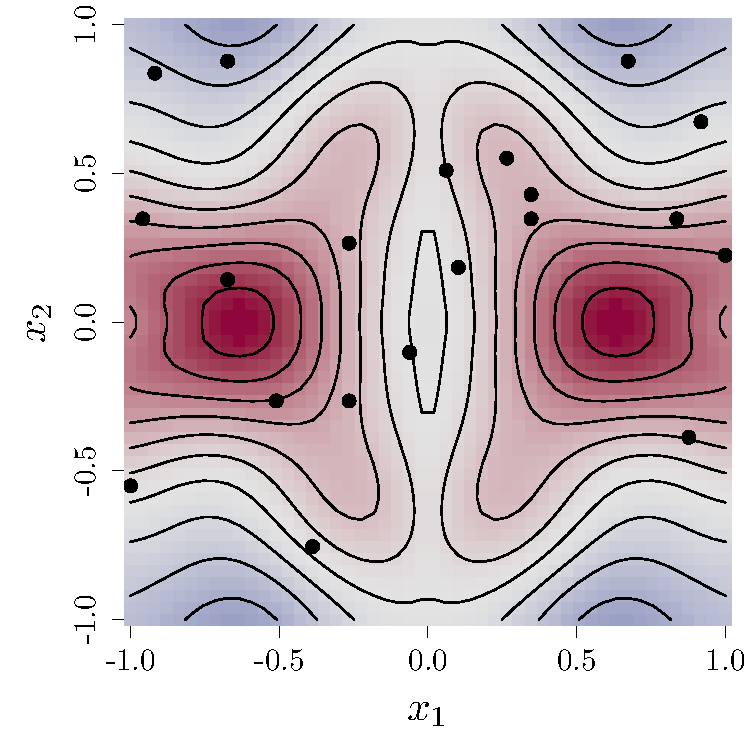
\includegraphics[width=\textwidth]{figures/ch5_symmean}
                \caption{GPR predicted mean.}
        \end{subfigure}
        \hspace{0.2cm}       
        \begin{subfigure}[t]{0.30\textwidth}
                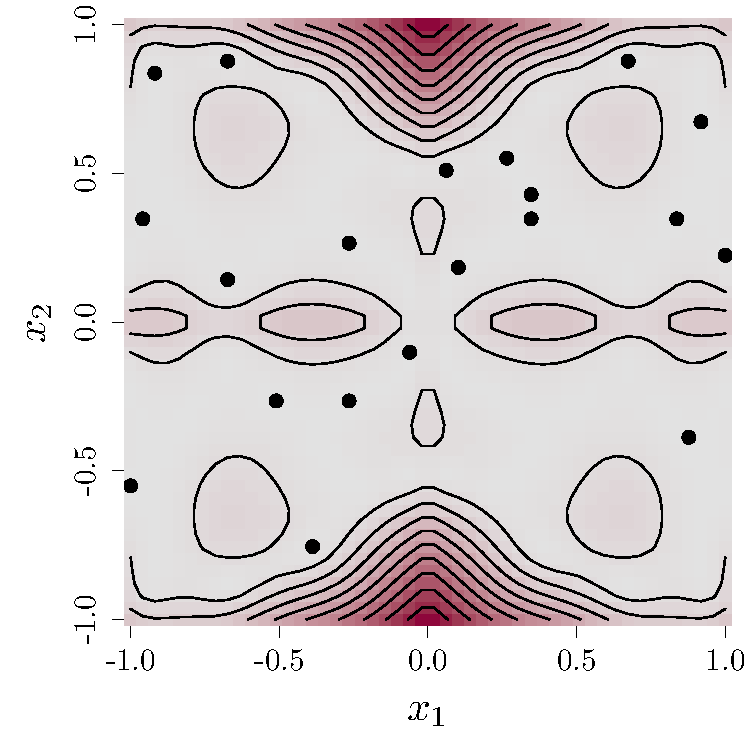
\includegraphics[width=\textwidth]{figures/ch5_symsd}
                \caption{GPR predicted standard deviation.}
        \end{subfigure}
        \caption{Examples of sample and GPR model generated with a kernel encapsulating symmetry information. The colour scale is different in each graph but blue colours always stand for negative values whereas red ones denote positive values.}
        \label{fig:ch5sym}
    \end{figure}
\end{example}

\begin{example}[Samples with zero integrals]
    In order to approximate a function over $D$ with integral equal to zero, one can think about building an appropriate kernel to encapsulate this information. The first application returning a centred function that comes to mind is:
    \begin{equation}
     L: \ f \rightarrow f - \int_D f(s) \dx s. 
    \end{equation}
     If we apply this transformation to a centred Gaussian process $Z$ with kernel $k$, we obtain a new Gaussian Process $Z_0(x) = Z(x) - \int_D Z(s) \dx s$ with kernel
     \begin{equation}
     \begin{split}         
     k_0(x,y) &= \Cov[Z_0(x),Z_0(y)] \\
     &= \Cov \left[ Z(x) - \int_D Z(s) \dx s,Z(y) - \int_D Z(s) \dx s \right] \\
     &= \Cov \left[Z(x),Z(y) \right] - \Cov \left[Z(x),\int_D Z(s) \dx s \right] - \Cov \left[\int_D Z(s) \dx s,Z(y) \right] \\
     & \qquad + \Cov \left[ \int_D Z(s) \dx s,\int_D Z(s) \dx s \right] \\
     &= k(x,y) - \int_D k(x,s) \dx s - \int_D k(y,s) \dx s + \iint_{D^2} k(s,t) \dx s \dx t
     \end{split}
    \end{equation}
    When using such kernel, the integral of each sample will be exactly zero.
\end{example}

In these two examples, it was easy to find an application that projects any function to the space of functions with the desired properties. However, such mapping is not unique and one could think about many other ways to symmetrise a function with respect to both axis such as $L(f)(x) = 1/4 \big( f(x_1,x_2) + f(-x_1,x_2) + f(x_1,-x_2) + f(-x_1,-x_2) \big)$. Of course, one of these operators is more suited to encapsulate the symmetry information. For the null integral example, it can be proven that the optimal centring operator is
\begin{equation}
     L(f)(x) \rightarrow f(x) - \frac{\displaystyle \int_D f(s) \dx s \int_D k(x,s) \dx s}{\displaystyle \iint_{D^2} k(s,t) \dx s \dx t}. 
\end{equation}
This can be proved by computing the distribution of $Z(x)|\int_D f(s) \dx s  \shorteq  0$. However, there is no general answer on how to find the appropriate projection of any prior knowledge. 

%%%%%%%%%%%%%%%%%%%%%%%%%%%%%%%%%%%%%%%%%%%%%%%%%%%%%%%%%%%%
\chapter*{Conclusion}
\addcontentsline{toc}{chapter}{Conclusion}

\paragraph{}
I have tried to encapsulate in this document the most important properties of Gaussian process regression models. This overview may seems either superficial for someone interested in the theory of Gaussian processes and too mathematical for a user mainly focussed on the applications of these models. However, I am convinced that someone with a good understanding of this document will be able to successfully use Gaussian process regression methods on real life data. In the end, the best way to learn about modelling is to use these methods and to practice on various datasets. For this sake, some available packages such as \emph{DiceKriging} in R or \emph{GPy} in Python can be of great help. 

\paragraph{}
Various subjects have been omitted in this document, such as the theory of Gaussian process regression with trend (Universal Kriging) or the variogram theory for parameter estimation but I have always tried to include alternative approaches that have their own advantage: for example, including trend can be done by adding a kernel with large length scale. Among the important subjects that have not been been mentioned we can cite the fundamental link between Gaussian Process regression and many other modelling methods such as linear regression, splines models or Kalman filters.

\paragraph{}
Future versions of this document will probably contain more references to the literature for readers interested in more details on specific topics. In the meantime, I can recommend one of the books that strongly participated to my interest in this field: \emph{Gaussian Processes For Machine Learning}\footnote{This book has been published by the MIT press in 2006 and it is available for free online at http://www.gaussianprocess.org/gpml} from Carl Edward Rasmussen and Christopher K. I. Williams.

\end{document}
